% =====================================================================
%  2026 高教社杯全国大学生数学建模竞赛  A 题  药材的烘干问题
%  【纸质版 / 打印版】包含承诺书与编号专用页
%  编译：xelatex paper.tex （或 latexmk -xelatex paper）
%  电子版请改用 paper_electronic.tex（第一页即摘要页）
% =====================================================================
% !TeX program = xelatex
\documentclass{cumcmthesis}

\usepackage{amsmath,amssymb,bm}
\usepackage{booktabs}
\usepackage{graphicx}
\usepackage{subcaption}
\usepackage{listings}
\usepackage{xcolor}
\usepackage{url}
\usepackage{array}
\usepackage{longtable}

\hypersetup{pdftitle={药材的烘干问题}, pdfauthor={}, unicode=true}

% 版面压缩：正文页数上限为 30 页（格式规范第四条）
\setlength{\textfloatsep}{3pt plus 1pt minus 1pt}
\setlength{\floatsep}{3pt plus 1pt minus 1pt}
\setlength{\intextsep}{3pt plus 1pt minus 1pt}
% 题注上下留白：默认 \abovecaptionskip=10pt，收紧后每幅图/表省 7pt
\setlength{\abovecaptionskip}{3pt}
\setlength{\belowcaptionskip}{2pt}

% ---- 代码清单样式 -------------------------------------------------
\definecolor{lstbg}{RGB}{248,248,248}
\definecolor{lstcmt}{RGB}{0,128,0}
\definecolor{lstkw}{RGB}{0,0,200}
\lstset{
  language=Python,
  backgroundcolor=\color{lstbg},
  basicstyle=\ttfamily\fontsize{6.6}{7.6}\selectfont,
  keywordstyle=\color{lstkw}\bfseries,
  commentstyle=\color{lstcmt},
  stringstyle=\color{red!70!black},
  numbers=left,
  numberstyle=\ttfamily\fontsize{5.5}{6.5}\selectfont\color{gray},
  numbersep=5pt,
  frame=single,
  rulecolor=\color{gray!45},
  breaklines=true,
  breakatwhitespace=false,
  postbreak=\mbox{\textcolor{gray}{$\hookrightarrow$}\space},
  columns=flexible,
  keepspaces=true,
  showstringspaces=false,
  extendedchars=true,
  tabsize=4,
  xleftmargin=14pt,
  framexleftmargin=14pt,
  captionpos=b,
}

% ---- 封面信息（纸质版打印后手写填入，电子版不出现本页） -----------
\title{药材的烘干问题}
\tihao{A}
\baominghao{}
\schoolname{}
\membera{}
\memberb{}
\memberc{}
\supervisor{}
\yearinput{2026}
\monthinput{9}
\dayinput{}

\begin{document}
\maketitle

% =====================================================================
%  CUMCM 2026 A 题  药材的烘干问题
%  正文与附录主体（由 paper.tex / paper_electronic.tex 共同 \input）
%  编译：xelatex（必须）
% =====================================================================

\begin{abstract}
中药材热风烘干是典型的「热湿耦合传递 + 相变 + 尺寸收缩」问题。本文以圆柱形药材为
对象，从壳层守恒出发建立温度--水分浓度耦合的轴对称扩散方程组，用保质量的有限体积
/Crank--Nicolson 格式求解，并以多种数值实现与解析解交叉验证。

\textbf{针对问题一}，将长径比 $L/R=12.5$ 的药材简化为无限长圆柱的一维径向问题，由
Fourier 定律与 Fick 定律推得
$\rho c_p\partial_tT=r^{-1}\partial_r(rk\partial_rT)$ 与
$\partial_tC=r^{-1}\partial_r(rD(C)\partial_rC)$，边界取 Robin 条件。先对附件 1 的
实测环境做一阶惯性拟合（$T_{air}$ 的 $R^2=0.9957$，RMSE $=0.336\,^\circ$C），
再以 1600 个控制体、$\Delta t=1$ s 求解：$1800$ s 时中心温度升至
$34.0425\,^\circ$C、表面 $37.1989\,^\circ$C，中心水分浓度仍为 $2.5500$ kg/kg、
表面降至 $1.5109$ kg/kg，截面平均含水由 $2.5500$ 降到 $2.2907$ kg/kg；
干物质质量 $72.57$ g（按附录 2 的 $\rho=820$ kg/m$^3$），1800 s 内脱除水分
$18.71$ g（占初始水量 $10.1\%$）。传质 Fourier 数仅 $0.0222$，
说明该阶段以升温为主、失水集中在表层。

\textbf{针对问题二}，改用附录 3 的变物性关系，并按题意把工艺分为预热平衡
（$0\sim4$ h）与恒温干燥（$t>4$ h，$T_{air}=50.212\,^\circ$C、$C_{air}=0.0509$ kg/kg）
两个阶段。3 h 内中心温升到 $49.9051\,^\circ$C、近似与环境平衡；水分浓度由表及里
依次下降，3 h 时中心 $1.7673$、表面 $1.0083$ kg/kg。

\textbf{针对问题三}，以「处处低于 $0.15$ kg/kg」为判据，指出中心是最后干燥点，
经网格加密与 Richardson 外推得
$\boxed{t_{dry}=205559\ \mathrm{s}=57.10\ \mathrm{h}=2.38\ \mathrm{d}}$，
与题目「一般持续 2--3 天」一致；此时截面平均含水 $0.1232$ kg/kg。

\textbf{针对问题四}，引入物质坐标 $\xi=r/R(t)$，严格导出各向同性收缩下无对流项的
Lagrangian 形式 $\partial_tC=(\xi R^2)^{-1}\partial_\xi(\xi D\partial_\xi C)$，
并用附件 2 的实测 $R(t)$（$2.000\to1.198$ cm）求得
$\boxed{t_{dry}=182765\ \mathrm{s}=50.77\ \mathrm{h}=2.12\ \mathrm{d}}$。
表格距离列取\textbf{当前物理距离} $r$（按 $\xi=r_j/R(t_i)$ 采样、
$r_j>R(t_i)$ 留空）；忽略收缩会把烘干时间高估 $2.5$ 倍。外部校验发现附件 2 的
收缩数据与附录 4 的密度式在干基质量守恒下最大不自洽 $17.8\%$。

\textbf{模型检验}：与 Bessel 级数解析解相比全场最大偏差 $1.0\times10^{-3}$ K、
中心点 $1.2\times10^{-5}$ K；空间与时间收敛阶均为二阶（$N=100\to800$ 误差降
$91$ 倍，$\Delta t=4\to0.25$ s 降 $195$ 倍）。三组数值实现（节点／单元中心有限
体积、直线法）在 $t=2.0\times10^5$ s 的中心含水相差不超过 $0.0066\%$，其中前两者
是两种\textbf{不同的空间离散}；水分守恒残差 $2.1\times10^{-5}$。灵敏度分析表明
\textbf{活化温度 3850 K 主导不确定性}（$\pm2\%\to\pm24\%$），浓度指数次之
（$\pm5\%$）。

\keywords{热湿耦合扩散；变物性；Robin 边界；收缩介质物质坐标；有限体积法；
Richardson 外推；灵敏度分析}
\end{abstract}

% =====================================================================
\section{问题重述}

\subsection{问题背景}

干燥是中药材产地加工与炮制过程中的关键工序，直接决定成品的有效成分保留率、
外观等级与贮藏稳定性；热风烘干因设备简单、成本低，是目前使用最广的干燥方式
之一\cite{li2024,zhang2022}。该过程包含两个阶段：先是\textbf{预热平衡阶段}，药材由环境
温度被加热到接近烘房温度、内部建立起稳定的温度梯度；随后进入\textbf{恒温干燥
阶段}，在近似恒定的温湿度环境下水分由内部迁至表面并被气流带走。工艺参数选择
不当会导致干燥过慢（能耗高、周期长）、表面「结壳」（外干内湿）或温度过高
（破坏热敏性成分），而传统的「试错--检测」优化模式周期长、成本高，因此有必要
用数理模型刻画药材内部温度与水分浓度的时空演化，以预测干燥时长、指导工艺设计。

本题的对象是一根形状近似为圆柱的中药材：长 $25$ cm、半径 $2$ cm，初始温度
$28\,^\circ$C，初始干基含水率 $2.55$ kg/kg。烘房温度与水分浓度的时间序列由
附件 1 给出，药材在干燥过程中的半径变化由附件 2 给出，问题 1--4 所需的物性
经验关系分别由附录 2--4 给出。

\subsection{需要解决的问题}

\begin{itemize}
  \item \textbf{问题一}：建立\textbf{预热平衡阶段}药材温度与水分浓度变化规律的数学模型
  （参数取附录 2），给出 $t=100,300,600,900,1200,1500,1800$ s、$r=0,0.5,1,1.5,2$ cm
  处的温湿度结果，并将 $1800$ s 内每 $1$ s、径向每 $0.1$ cm 的完整结果写入
  \texttt{result1.xlsx}。
  \item \textbf{问题二}：建立\textbf{整个烘干过程}（约 2--3 天）的数学模型，物性统一取
  附录 3，给出 3 h 内每 $0.5$ h、上述五个半径处的结果，并把每 $1$ s、径向每
  $0.1$ cm 的完整结果写入 \texttt{result2.xlsx}。
  \item \textbf{问题三}：以「药材各处水分浓度均低于 $0.15$ kg/kg」为烘干判据，
  确定所需烘干时间（单位 h），给出每 $6$ h、径向每 $0.5$ cm 的水分浓度，并把
  每 $60$ s、径向每 $0.1$ cm 的完整结果写入 \texttt{result3.xlsx}。
  \item \textbf{问题四}：考虑干燥过程中药材因失水而发生的\textbf{尺寸收缩}
  （半径历史见附件 2，物性取附录 4），重新确定烘干时长，给出每 $6$ h、径向每
  $0.5$ cm 的水分浓度（末列为随时间移动的药材表面），并把每 $60$ s、径向每
  $0.1$ cm 的完整结果写入 \texttt{result4.xlsx}。
\end{itemize}

每个问题都需要明确三件事：\textbf{输入}（初始温湿度、烘房环境时间序列、物性关系、
几何尺寸）、\textbf{输出}（规定时刻与位置的温度与水分浓度）、\textbf{判定标准}
（问题 1--2 为数值结果的精度与守恒性；问题 3--4 为「处处低于 $0.15$ kg/kg」这一
判据首次被满足的时刻）。

% =====================================================================
\section{问题分析}

\subsection{为什么是「耦合扩散」而不是「经验干燥曲线」}

中药材的干燥在机理上同时包含三个过程：热量由热风经表面对流进入药材内部
（Fourier 导热）、水分以液态扩散的形式由内部向表面迁移（Fick 扩散）、以及
表面发生的对流传质\cite{mujumdar2014,chaedir2019}。三者由\textbf{材料内部的
温湿度场}耦合在一起：附录的经验关系表明扩散系数 $D$ 同时依赖水分浓度 $C$ 与
温度 $T$（Arrhenius 形式），而 $\rho$、$c_p$、$k$ 又都依赖 $C$。

因此，薄层干燥经验模型（如 Page 模型、Weibull 模型）虽然能拟合整体的含水率--
时间曲线，却\textbf{无法回答本题的核心问题}：题目要求给出「到药材中心不同距离
处」的温度与水分浓度，而经验模型只描述截面平均量、缺少空间分辨率，无法判定
「处处低于 $0.15$ kg/kg」这一内部判据。故必须建立分布参数模型。

理由链可以完整表述为：

\begin{center}
\begin{tabular}{p{0.20\textwidth}p{0.70\textwidth}}
\toprule[1.2pt]
\textbf{环节} & \textbf{内容} \\
\midrule
机理 & 表面受对流换热与对流传质控制；内部受导热与水分扩散控制；物性随 $C,T$ 变化 \\
模型形式 & 轴对称非稳态扩散方程组（抛物型 PDE）+ Robin 边界 + 变系数耦合 \\
可辨识参数 & $\rho,c_p,k,D$ 由附录经验式给出；$h=25\ \mathrm{W/(m^2K)}$、
  $h_m=8\times10^{-7}$ m/s 由附录 2 给出；环境由附件 1 给出 \\
求解方法 & 归一化半径上的有限体积离散 + $\theta$ 法时间推进（$\theta=1/2$ 即
  Crank--Nicolson），三对角线性系统用 LAPACK 带状求解器 \\
可验证性 & 常物性恒环境条件下存在 Bessel 级数解析解；离散格式严格守恒，可做
  水分总量核对；可与降维模型、直线法对照 \\
\bottomrule[1.2pt]
\end{tabular}
\end{center}

\subsection{问题一的分析}

预热平衡阶段只有 $1800$ s。由附录 2 可估算两个特征时间：
热扩散时间 $\tau_T=R^2/\alpha=R^2\rho c_p/k=2369$ s，水分扩散时间
$\tau_D=R^2/D(C_0)=8.1\times10^4$ s。二者相差 34 倍，说明\textbf{在 30 分钟内
温度场会发生显著变化，而水分场只能在表层发生可观测的改变}。这一数量级判断
直接决定了结果形态，也为后续结果合理性检查提供了先验依据。

另一个关键点是\textbf{附件 1 的处理}。附件 1 是带噪声的实测环境序列（241 个
点，采样间隔 60 s），若直接把它作为边界条件会引入阶跃噪声。本文先做一阶惯性
拟合（$T_{air}=T_{set}-(T_{set}-28)e^{-t/\tau_T}$），并把「用拟合曲线」与
「用附件 1 原始插值」两种口径都算过：对 $t_{dry}$ 而言两者只差 $0.12$ h
（$0.2\%$）；但对问题 1 的 30 分钟温度表，拟合曲线在 $60\!\sim\!2300$ s
（$1\!\sim\!38$ min）内\textbf{系统性高于实测，最大偏高 $0.96\,^\circ$C}
（残差滞后 1 阶自相关达 $0.83$，
说明它不只是随机噪声，而是模型形式失配），使表~\ref{tab:p1T} 各值系统性偏高，
最大偏高 $0.52\,^\circ$C（$t=1200$ s、$r=2.0$ cm 处）。本文因此
\textbf{如实报告两种口径}（对照见 10.7 节表~\ref{tab:p1env}）：正文
表~\ref{tab:p1T}、表~\ref{tab:p1C} 取拟合边界，并明确其代价。

\subsection{问题二与问题三的分析}

问题二的时间尺度跃升到 2--3 天，出现了两个新问题。其一，\textbf{物性不再是
常数}：附录 3 的 $D$ 随 $C$ 呈 $\exp(-a/C)$ 下降（$C$ 由 $2.55$ 降到 $0.15$
时降近一个数量级），又对温度呈 $\exp(-3850/T)$ 的强依赖，方程因此\textbf{强
非线性}，干燥后期进入「降速干燥」区，常系数近似会带来系统性偏差。其二，
\textbf{需区分两个工艺阶段}：题目指出两阶段「参数有所不同」，而附件 1 显示
烘房在 4 h 左右达到 $50.2\,^\circ$C 并稳定，故本文取 $0\sim4$ h 为预热平衡
阶段（环境按附件 1 上升）、$t>4$ h 为恒温干燥阶段（$T_{air}=50.212\,^\circ$C、
$C_{air}=0.0509$ kg/kg）。

问题三的关键判断是：\textbf{判据「处处低于 0.15 kg/kg」由中心点最后满足}——
圆柱几何下中心是扩散路径最长的点。本文不预设这一点，而是逐时刻搜索
$\max_r C(r,t)$ 及其位置，用数据确认最大值始终位于中心（8.1 节）。

\subsection{问题四的分析}

尺寸收缩给模型带来两个变化：求解域 $[0,R(t)]$ 是\textbf{移动边界}，且材料点
随收缩向轴心移动。若在固定物理坐标下用移动网格求解，需在方程中显式加入对流项，
边界处理复杂且易引入数值耗散。

本文采用\textbf{物质坐标（Lagrangian）变换} $\xi=r/R(t)$：对各向同性收缩，
每个材料点保持 $\xi$ 不变，由「以固定干基质量为控制体」的守恒推导（5.5 节）
可得水分方程在物质坐标下\textbf{对流项严格为零}：

\[
\frac{\partial C}{\partial t}=\frac{1}{\xi R(t)^2}\frac{\partial}{\partial \xi}
\left(\xi D\frac{\partial C}{\partial \xi}\right),
\]

该式在 $R=\text{const}$ 时退化为问题 1--3 的标准圆柱扩散方程，形式统一、边界
固定，是本文处理收缩的主要手段。同时，附件 2 的半径历史与附录 4 的密度式之间
存在\textbf{可能的不自洽}（若严格守恒干基质量，由 $\rho(C)$ 反推的终态半径应
大于实测值）；本文遵守题面「根据附件 2 确定烘干时长」的指令直接使用实测
$R(t)$，并把这一不自洽量化为一条独立的模型检验结论（10.6 节）。

% =====================================================================
\section{模型假设}

\begin{enumerate}
  \item \textbf{无限长圆柱}：药材长 $25$ cm、半径 $2$ cm，长径比 $12.5$，且气流
  沿轴向均匀，故忽略轴向与端面效应，问题化为轴对称一维径向问题。\textit{条件}：
  $L/R\gg1$。
    \item \textbf{局部热力学平衡}：固相与液相同温；水分迁移由单一有效扩散系数
  $D(C,T)$ 描述，把毛细流动与蒸汽扩散两种机制合并为一个等效系数——这是对
  Luikov 双机制耦合模型的简化\cite{luikov1966}。\textit{条件}：
  $\mathrm{Le}=D/\alpha\ll1$（本文 $\mathrm{Le}\sim10^{-2}\!\sim\!10^{-1}$）。
\item \textbf{常压、无内热源}：烘房为常压通风环境，不计压缩功与黏性耗散，
  内部无体积热源。
  \item \textbf{表面传热传质系数为常数}：$h=25$ W/(m$^2$K)、
  $h_m=8\times10^{-7}$ m/s 由气流状态决定，不随时间与含水率变化。
  \item \textbf{水分以干基浓度描述}：$C$ 为「每千克干物质所含的水分质量」，
  干物质不迁移，故水分守恒方程以固定干基质量为控制体自然成立。
  \item \textbf{各向同性收缩（仅问题四）}：同一物质点恒满足 $r=\xi R(t)$，
  由此可推出物质坐标下无对流项。
  \item \textbf{恒温阶段环境恒定}：由附件 1，烘房 4 h 内达到设定值并稳定；恒温
  阶段视为已排湿的稳定工况，取 $T_{air}=50.212\,^\circ$C、
  $C_{air}=0.0509$ kg/kg。
  \item \textbf{基准模型不计蒸发潜热}：题面未给水的汽化潜热，而题给的
  $(h,h_m)$ 与热质比拟的 Lewis 关系相差 4 个数量级，潜热份额无法由题面数据
  判定（10.8 节给出论证），故基准模型不含该项。
\end{enumerate}

% =====================================================================
\section{符号说明}

% 本表共 24 行，仍超过一页的文本高度，必须用可跨页断开的 longtable，
% 否则 tabular 会溢出到页面之外并把页脚页码挤掉。
{\small
\setlength{\LTpre}{3pt}
\setlength{\LTpost}{3pt}
\renewcommand{\arraystretch}{0.98}
\begin{longtable}{clc}
\toprule[1.5pt]
\makebox[0.16\textwidth][c]{符号} & \makebox[0.58\textwidth][c]{意义} &
\makebox[0.18\textwidth][c]{单位} \\
\midrule[1pt]
\endfirsthead
\multicolumn{3}{r}{\small（续）}\\
\toprule[1.5pt]
\makebox[0.16\textwidth][c]{符号} & \makebox[0.58\textwidth][c]{意义} &
\makebox[0.18\textwidth][c]{单位} \\
\midrule[1pt]
\endhead
\bottomrule[1.5pt]
\endfoot
$r$        & 到药材中心的距离（物理坐标） & m \\
$R(t)$     & 药材半径（问题四中随时间变化） & m \\
$R_0,\,L$  & 初始半径与药材长度，$0.02$ / $0.25$ & m \\
$\xi$      & 归一化/物质半径，$\xi=r/R(t)$ & --- \\
$t$        & 时间 & s \\
$T(r,t)$   & 药材温度 & $^\circ$C \\
$T_{air}(t)$ & 烘房空气温度 & $^\circ$C \\
$T_{set},\,C_{set}$ & 恒温阶段的设定温度与含湿量，$50.212$ / $0.050908$ & $^\circ$C, kg/kg \\
$C(r,t)$   & 干基水分浓度 & kg/kg \\
$C_{air}(t)$ & 烘房空气水分浓度（含湿量） & kg/kg \\
$\rho(C)$  & 药材密度 & kg/m$^3$ \\
$c_p(C)$   & 药材比热容 & J/(kg$\cdot$K) \\
$k(C)$     & 热传导系数 & W/(m$\cdot$K) \\
$D(C,T)$   & 水分浓度扩散系数 & m$^2$/s \\
$h$        & 对流换热系数，$25$ & W/(m$^2\cdot$K) \\
$h_m$      & 对流传质系数，$8\times10^{-7}$ & m/s \\
$\alpha$   & 热扩散率 $\alpha=k/(\rho c_p)$ & m$^2$/s \\
$Bi,\,Bi_m$ & 热/传质 Biot 数 $hR/k$、$h_mR/D$ & --- \\
$Fo,\,\mathrm{Le}$ & Fourier 数 $\alpha t/R^2$、Lewis 数 $D/\alpha$ & --- \\
$\tau_T,\tau_D$ & 热扩散、水分扩散特征时间 & s \\
$\mu_1,\,\lambda_1$ & 圆柱第一特征值（$\mu J_1=\!Bi_mJ_0$ 的最小正根）及其衰减率 $\mu_1^2D/R^2$ & ---, s$^{-1}$ \\
$t_{dry}$  & 烘干时间（判据首次满足的时刻） & s 或 h \\
$q_r$      & 径向通量（热或质） & W/m$^2$ 或 kg/(m$^2$s) \\
$\rho_d$     & 干基密度 $\rho/(1+C)$（单位湿体积内的干物质质量） & kg/m$^3$ \\
\end{longtable}
}
% longtable.sty executes \@kernel@refstepcounter{\LTcaptype} at \begin{longtable},
% which consumes one step of the table counter.  Without this reset the first
% real table of the paper would be numbered "表 2" and every later table would
% be off by one, so the numbering is put back to zero here.
\setcounter{table}{0}

% =====================================================================
\section{模型的建立}

\subsection{几何简化：由三维到一维}

药材为半径 $R_0=2$ cm、长 $L=25$ cm 的圆柱，长径比 $L/R_0=12.5$。轴向导热
特征时间为 $L^2/\alpha=0.25^2/1.6886\times10^{-7}\approx3.70\times10^5$ s
（约 $4.3$ 天），径向为 $R_0^2/\alpha\approx2369$ s，两者之比为
$(L/R_0)^2=156$，即相差约 $2.2$ 个数量级；同时烘房气流沿轴向均匀送风。
因此端面效应与轴向梯度可以忽略，
温度与水分浓度只依赖 $r$ 与 $t$，问题化为\textbf{轴对称一维径向}问题
（图~\ref{fig:schematic}）。

\begin{figure}[htbp]
  \centering
  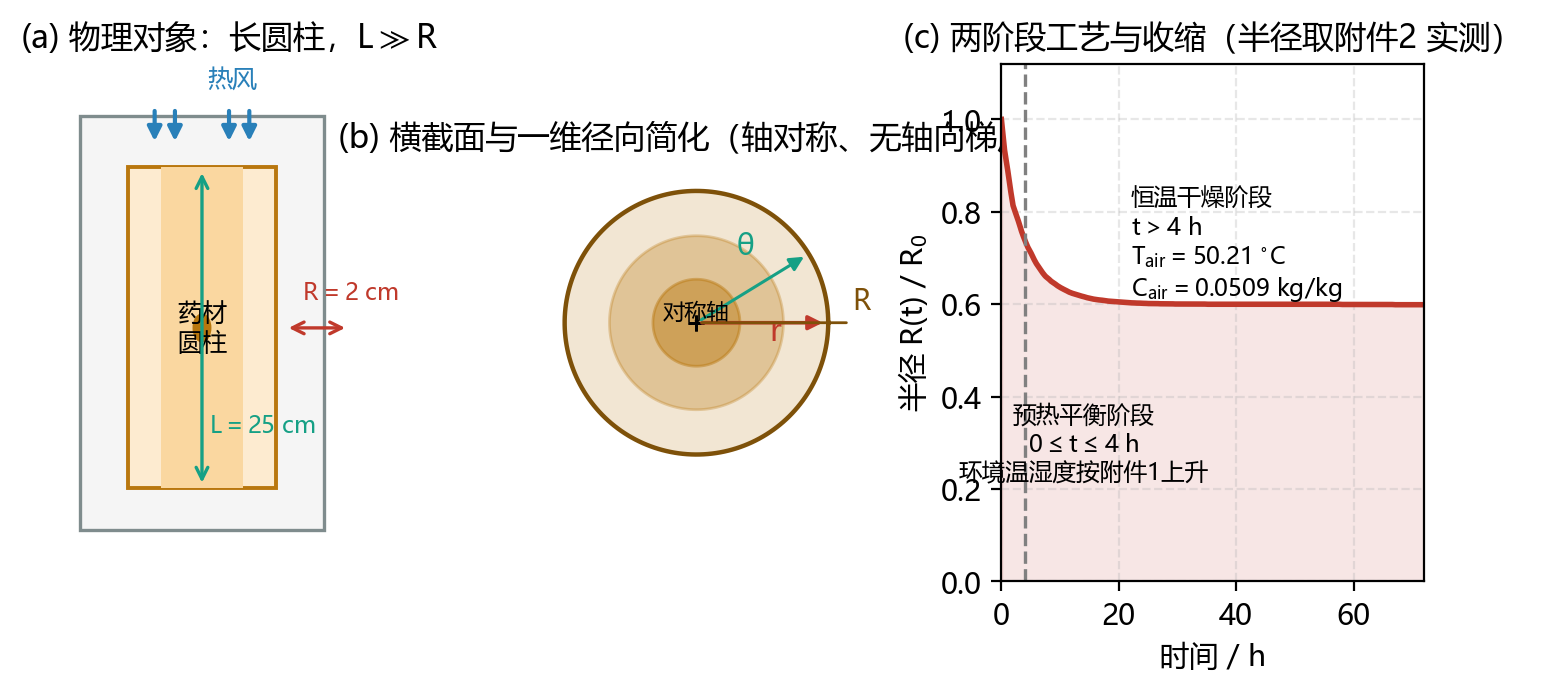
\includegraphics[width=0.84\textwidth]{figures/fig20_schematic.png}
  \caption{药材热风烘干问题的建模示意图：(a) 物理对象；(b) 横截面与一维径向简化；
  (c) 两阶段工艺与尺寸收缩}
  \label{fig:schematic}
\end{figure}

\subsection{传热控制方程}

在半径 $r$ 处取厚度 $\mathrm{d}r$、长 $L$ 的环形壳层。壳层内能的时变率等于
净导入的导热热流：

\[
\rho c_p\,(2\pi r L\,\mathrm{d}r)\frac{\partial T}{\partial t}
=-\Big[q_r\cdot 2\pi rL\Big]_{r}^{r+\mathrm{d}r},
\qquad q_r=-k\frac{\partial T}{\partial r},
\]

整理得圆柱坐标下的非稳态导热方程

\begin{equation}
\rho(C)\,c_p(C)\,\frac{\partial T}{\partial t}
=\frac{1}{r}\frac{\partial}{\partial r}\left(r\,k(C)\frac{\partial T}{\partial r}\right).
\label{eq:heat}
\end{equation}

\subsection{传质控制方程}

同一壳层内水分的时变率等于净导入的扩散质流。以干基浓度 $C$ 为变量，水分的
质量通量为 $j_r=-\rho_{d}D\,\partial C/\partial r$，其中 $\rho_d=\rho/(1+C)$ 为
单位湿体积内的干物质质量。注意到壳层内的干物质质量 $2\pi rL\rho_d\,\mathrm{d}r$
不随时间变化，对水分做守恒可得

\begin{equation}
\frac{\partial C}{\partial t}
=\frac{1}{r}\frac{\partial}{\partial r}\left(r\,D(C,T)\frac{\partial C}{\partial r}\right).
\label{eq:mass}
\end{equation}

式~\eqref{eq:mass} 的物理含义是：$C$ 是「每千克干物质的水量」，控制体随干物质
一起运动，因此方程中不含干物质密度的散度项，这也是后文处理收缩时的出发点。

\subsection{边界条件与初始条件}

\textbf{中心对称条件}（$r=0$）：

\begin{equation}
\left.\frac{\partial T}{\partial r}\right|_{r=0}=0,\qquad
\left.\frac{\partial C}{\partial r}\right|_{r=0}=0 .
\end{equation}

\textbf{表面 Robin 条件}（$r=R$，$n$ 取外法向）\cite{incropera2007}。热量由
热风以对流方式传入、水分由表面以对流方式带出：

\begin{equation}
-k\left.\frac{\partial T}{\partial r}\right|_{r=R}=h\left(T_s-T_{air}(t)\right),
\qquad
-D\left.\frac{\partial C}{\partial r}\right|_{r=R}=h_m\left(C_s-C_{air}(t)\right),
\label{eq:robin}
\end{equation}

其中 $T_s=T(R,t)$、$C_s=C(R,t)$。两式左端都是「向外法向的通量」，故 $T_{air}>T_s$
时导热项为负（热量向内传入），与 5.5 节的物质坐标形式的表面条件一致。

\textbf{初始条件}：

\begin{equation}
T(r,0)=28\,^\circ\mathrm{C},\qquad C(r,0)=2.55\ \mathrm{kg/kg},\qquad 0\le r\le R_0 .
\end{equation}

\subsection{收缩问题的物质坐标变换}

当 $R=R(t)$ 时，求解域随时间变化。引入物质坐标

\begin{equation}
\xi=\frac{r}{R(t)}\in[0,1],\qquad r=\xi R(t).
\end{equation}

对各向同性收缩，同一物质点在任意时刻满足 $r(t)=\xi R(t)$，即 $\xi$ 是材料标签。
干燥过程中干物质本身不迁移，故任一材料壳层 $[\xi,\xi+\mathrm{d}\xi]$ 所含的
干物质质量守恒。该壳层在当前构形下的体积（单位长度）为
$2\pi r\,\mathrm{d}r=2\pi R^2\xi\,\mathrm{d}\xi$，于是

\begin{equation}
\frac{\partial}{\partial t}\Big(\rho_d\,\xi R^2\Big)\Big|_{\xi}=0
\quad\Longrightarrow\quad
\rho_d(\xi,t)\,R(t)^2=\rho_d(\xi,0)\,R_0^2 ,
\label{eq:dryinv}
\end{equation}

即 $\rho_dR^2$ 是材料不变量——这是移动边界问题在物质坐标下的一个关键性质。

再对固定的材料区域 $[0,\xi]$ 做水分衡算。区域内水分只经由 $\xi$ 处的材料面与
外界交换：以干物质计的扩散质流密度为
$j_r=-\rho_dD\,\partial C/\partial r=-(\rho_dD/R)\,\partial C/\partial \xi$，
材料面面积（单位长度）为 $2\pi\xi R$。注意到区域内的干物质质量
$\mathrm{d}m_d=\rho_d\,2\pi R^2\xi'\,\mathrm{d}\xi'$ 不随时间改变，其中的水分
质量 $C\,\mathrm{d}m_d$ 的变化率即为 $\mathrm{d}m_d\,\partial_tC$，故

\begin{equation}
2\pi R^2\!\!\int_0^{\xi}\!\rho_d\,\xi'\,
\frac{\partial C}{\partial t}\,\mathrm{d}\xi'
=-\big(j_r\cdot2\pi\xi R\big)
=2\pi\,\xi\,\rho_d D\,\frac{\partial C}{\partial \xi}.
\end{equation}

两边对 $\xi$ 求导并约去公因子 $2\pi$，得物质坐标下的\textbf{一般形式}

\begin{equation}
\frac{\partial C}{\partial t}\bigg|_{\xi}
=\frac{1}{\xi R(t)^2\rho_d}\frac{\partial}{\partial \xi}
\left(\xi\,\rho_d D\frac{\partial C}{\partial \xi}\right).
\label{eq:shrink-general}
\end{equation}

由式~\eqref{eq:dryinv}，$\rho_d$ 沿 $\xi$ 的分布不随时间改变；而初始时刻
$C\equiv2.55$ kg/kg 处处相等，故 $\rho_d(\xi,0)$ 为常数。因此 $\rho_d$ 在
干燥全程都与 $\xi$ 无关，可从式~\eqref{eq:shrink-general} 中当作常数约去，
得到本文实际使用的形式

\begin{equation}
\boxed{\ \frac{\partial C}{\partial t}
=\frac{1}{\xi R(t)^2}\frac{\partial}{\partial \xi}
\left(\xi D\frac{\partial C}{\partial \xi}\right)\ }
\label{eq:shrink}
\end{equation}

\textbf{对流项严格为零}。这是本文处理收缩的核心结论：只要收缩是各向同性的，
在物质坐标下移动边界问题就化为固定域问题，只需把 $R(t)$ 代入 Laplacian 的
系数即可，无需引入网格运动或 ALE 对流项。当 $R(t)=R_0$ 时式~\eqref{eq:shrink}
退化为式~\eqref{eq:mass}，说明问题 1--4 可用同一套代码框架求解。

\textbf{推导前提}。上述推导用到两条前提，它们在本工况下成立，但应显式写出以免
误用。\textbf{（一）干基密度与 $\xi$ 无关}：这不是近似，而是式~\eqref{eq:dryinv}
的直接推论——$\rho_dR^2$ 逐材料点守恒，而初始含水率均匀使
$\rho_d(\xi,0)=\rho(C_0)/(1+C_0)$ 为常数，故 $\rho_d$ 全程与 $\xi$ 无关；它随
时间单调增大（附录 4 下 $C$ 由 $2.55$ 降到 $0$ 时 $\rho_d$ 由 $278.7$ 升到
$760$ kg/m$^3$），但该变化只依赖 $R(t)$，在式~\eqref{eq:shrink-general} 中被
约去。反之，若认为干密度随剖面不均匀，式~\eqref{eq:shrink} 会多出一阶项
$\frac{D}{R^2}\partial_\xi C\,\partial_\xi\ln\rho_d$，这种读法与附件 2 的实测
$R(t)$ 不相容（峰值偏差 $17.8\%$，10.6 节），故式~\eqref{eq:shrink} 在本工况下
是\textbf{精确}的。\textbf{（二）能量方程的单位体积热容}：本文直接取附录 4 的
$\rho(C)c_p(C)$ 作式~\eqref{eq:heat-shrink} 的系数，略去了「显热随含水率下降」
带来的附加项。其量级由 10.8 节的两个变体界定：把 $\rho c_p$ 乘 $(R_0/R)^2$ 后
$t_{dry}$ 只变 $+0.055\%$，加入体积项为 $-0.49\%$，都远小于 $D(C,T)$ 标定的
$\pm24\%$——因为水分场在 $2$ h 后已准平衡，这些项只改变温度的\emph{响应速率}，
不改变准平衡分布。用于收缩更剧烈（$R/R_0\ll0.6$）或热响应更慢的工况时，
上述前提应重新评估。

热传导方程在物质坐标下同理写成

\begin{equation}
\rho(C)c_p(C)\frac{\partial T}{\partial t}
=\frac{1}{\xi R(t)^2}\frac{\partial}{\partial \xi}
\left(\xi k(C)\frac{\partial T}{\partial \xi}\right).
\label{eq:heat-shrink}
\end{equation}

表面条件式~\eqref{eq:robin} 在物质坐标下为

\begin{equation}
-\frac{k}{R}\left.\frac{\partial T}{\partial \xi}\right|_{\xi=1}
=h\left(T_s-T_{air}\right),\qquad
-\frac{D}{R}\left.\frac{\partial C}{\partial \xi}\right|_{\xi=1}
=h_m\left(C_s-C_{air}\right).
\end{equation}

\subsection{物性经验关系与适用范围}

按题意，问题 1 用附录 2 的常数物性，问题 2--3 用附录 3 的经验式，问题 4 用
附录 4 的经验式（图~\ref{fig:props}）：

\begin{center}
{\small
\begin{tabular}{llll}
\toprule[1.2pt]
  & 附录 2（问题 1） & 附录 3（问题 2、3） & 附录 4（问题 4） \\
\midrule
$\rho$ / (kg/m$^3$) & $820$ & $650+128C$ & $760+90C$ \\
$c_p$ / (J/(kg$\cdot$K)) & $2600$ & $1450+2736\dfrac{C}{C+1}$ & $1850+2150\dfrac{C}{C+1}$ \\
$k$ / (W/(m$\cdot$K)) & $0.36$ & $0.21+0.38\dfrac{C}{C+1}$ & $0.12+0.20\dfrac{C}{C+1}$ \\
$D$ / (m$^2$/s) & $7\times10^{-9}e^{-0.89/C}$ & $2.4\times10^{-3}e^{-0.45/C}e^{-3850/T}$ & $4.2\times10^{-4}e^{-0.30/C}e^{-3850/T}$ \\
\bottomrule[1.2pt]
\end{tabular}
}
\end{center}

式中 $T$ 必须取绝对温度（K）。附录 2 的 $\rho,c_p,k$ 是常数、$D$ 又只依赖 $C$，
故\textbf{问题 1 的温度场与水分场完全解耦}（这也是 10.7 节环境口径只影响表面
水分浓度的原因）；问题 2--4 中 $D$ 依赖 $T$，两场才真正耦合。

\begin{figure}[htbp]
  \centering
  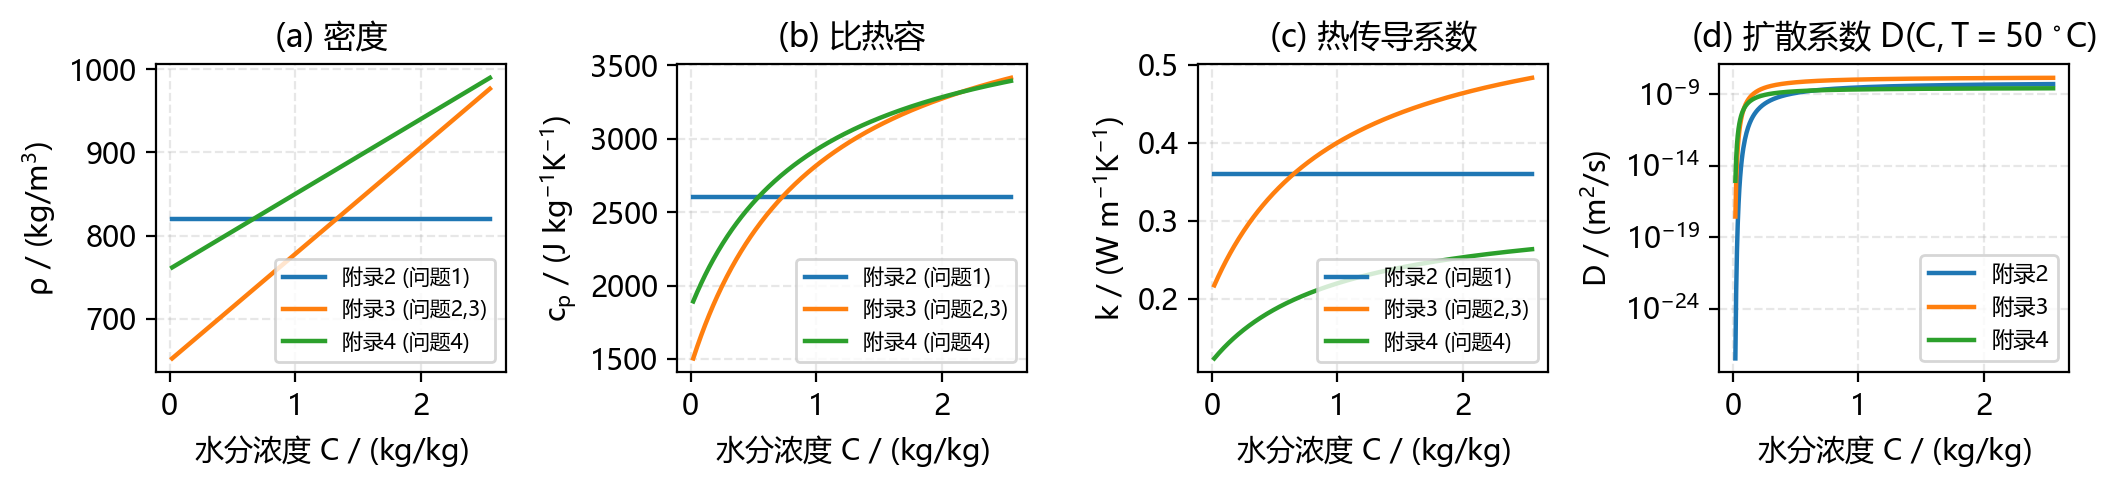
\includegraphics[width=0.84\textwidth]{figures/fig06_properties.png}
  \caption{附录给出的物性经验关系随水分浓度的变化}
  \label{fig:props}
\end{figure}

\textbf{量纲与数量级检查}。$e^{-3850/T}$ 是 Arrhenius 因子，对应活化能
$E_a=3850R_g=3850\times8.314=32.0$ kJ/mol（$R_g$ 为气体常数）；干燥中有效
水分扩散系数随温度呈 Arrhenius 形式是常用假设\cite{karatas1997}。
$e^{-a/C}$ 项则体现「随含水率下降扩散阻力急剧增大」的降速干燥特征。
由附录 3 计算：$C=2.55$、$T=50\,^\circ$C 时 $D=1.35\times10^{-8}$ m$^2$/s；
$C=0.15$ 时 $D=8.0\times10^{-10}$ m$^2$/s，下降 17 倍，说明\textbf{干燥后期
由内部扩散控制}。\textit{适用范围说明}：上述经验式由题目给定，其标定区间未在
题面说明；当 $C\to0$ 时 $e^{-a/C}\to0$，公式在极低含水率下会给出过小的 $D$，
本文据此在程序中设 $C\ge10^{-3}$ kg/kg 的下限保护，并在灵敏度分析中量化
$a$ 与 $3850$ 的不确定性影响。

\subsection{无量纲分析与工作量级的先验判断}

定义热 Biot 数、传质 Biot 数、Fourier 数与 Lewis 数：

\begin{equation}
Bi=\frac{hR_0}{k},\quad Bi_m=\frac{h_mR_0}{D},\quad
Fo=\frac{\alpha t}{R_0^2},\quad \mathrm{Le}=\frac{D}{\alpha}.
\end{equation}

\begin{itemize}
  \item 问题 1：$Bi=1.389$，$Bi_m=3.24$，$\mathrm{Le}=2.9\times10^{-2}$，
  $Fo_T(1800\,\mathrm{s})=0.760$，$Fo_D(1800\,\mathrm{s})=0.0222$。
  \item 问题 3（取 $C=2.55$、$T=50\,^\circ$C）：$D=1.347\times10^{-8}$ m$^2$/s，
  $\alpha=k/(\rho c_p)=0.4830/(976.4\times3415.3)=1.448\times10^{-7}$ m$^2$/s，
  $\mathrm{Le}=D/\alpha=0.093$，$Bi_m=h_mR_0/D=1.19$。
\end{itemize}

\textbf{两条先验结论}（图~\ref{fig:regime}）：第一，$Fo_D\ll Fo_T$，即温度先于
水分达到准平衡，因此问题 1 的 30 分钟内「水分几乎不动、温度显著上升」；
第二，$Bi_m$ 量级为 1，说明内部扩散与外部对流传质阻力\textbf{相当}，
不能简单地把表面当作平衡边界处理，必须保留 Robin 条件。

\begin{figure}[htbp]
  \centering
  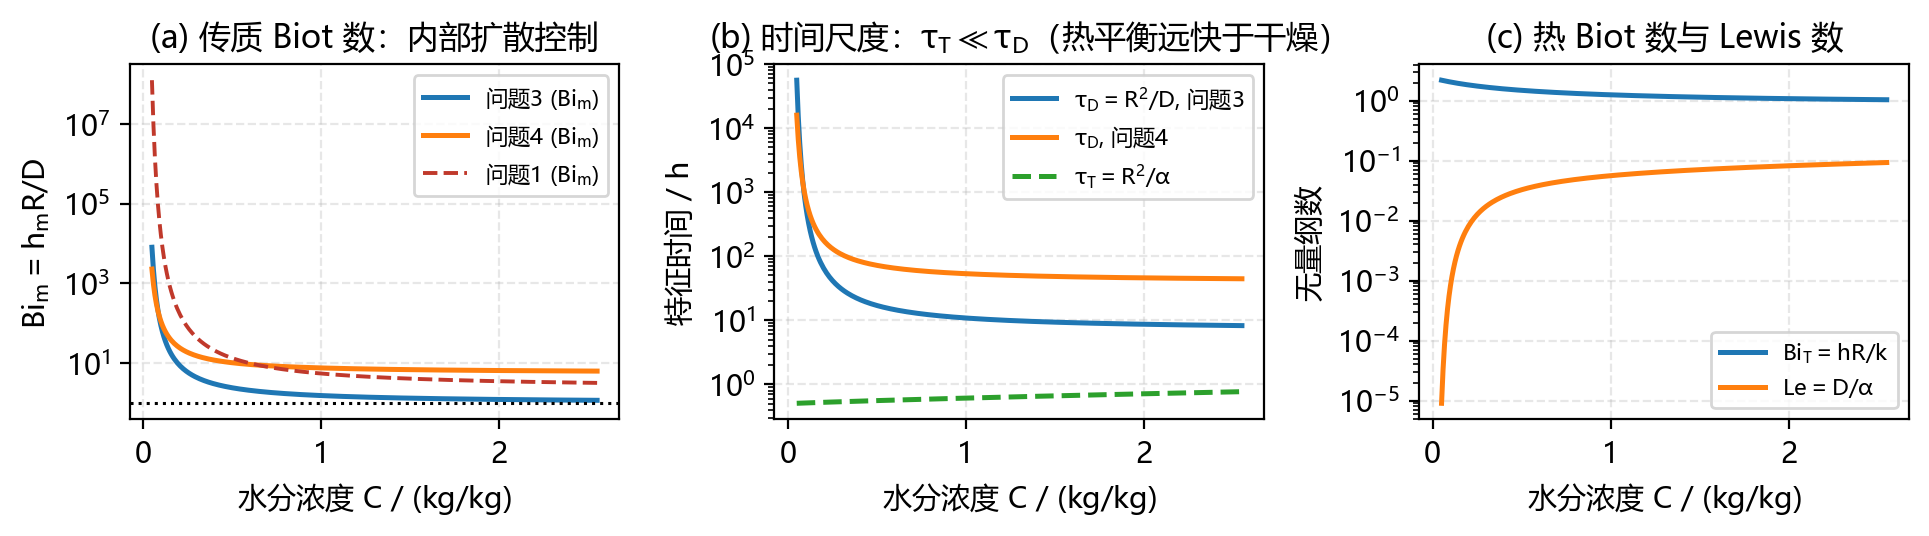
\includegraphics[width=0.84\textwidth]{figures/fig21_regime.png}
  \caption{无量纲分析：模型所处的工作区间。(a) 传质 Biot 数；(b) 各特征时间尺度；
  (c) 热 Biot 数与 Lewis 数}
  \label{fig:regime}
\end{figure}

\subsection{数值方法}

\textbf{空间离散}。在 $\xi\in[0,1]$ 上取 $N+1$ 个节点
$\xi_i=ih$，$h=1/N$，采用\textbf{节点中心有限体积}格式：节点 0 位于对称轴、
节点 $N$ 恰好位于药材表面。控制体取 $[0,h/2]$、$[\xi_i-h/2,\xi_i+h/2]$ 与
$[1-h/2,1]$，对应的体积测度为

\[
\mathrm{vol}_0=\frac{h^2}{8},\qquad
\mathrm{vol}_i=\xi_i h\ (1\le i\le N-1),\qquad
\mathrm{vol}_N=\frac{h}{2}-\frac{h^2}{8}.
\]

将式~\eqref{eq:shrink} 在控制体上积分，记面通量 $g=\xi D\partial_\xi C$，得

\begin{equation}
\frac{\mathrm{d}C_i}{\mathrm{d}t}
=\frac{1}{R^2\,\mathrm{vol}_i}\left(g_{i+\frac12}-g_{i-\frac12}\right),\qquad
g_{i+\frac12}=\frac{\xi_{i+\frac12}D_{i+\frac12}}{h}\left(C_{i+1}-C_i\right),
\end{equation}

其中面扩散系数取相邻两节点的\textbf{算术平均}
$D_{i+1/2}=(D_i+D_{i+1})/2$。表面面通量
由式~\eqref{eq:robin} 给出：$g_{N+\frac12}=-R\,h_m(C_N-C_{air})$；轴心处
$g_{-\frac12}=0$。该格式\textbf{逐项守恒}：对所有控制体求和可得水分总量的
变化率恰等于表面通量，误差仅为舍入误差。

\textbf{时间离散}。物性系数取上一时间步的显式值，未知量隐式处理，采用
$\theta$ 法：

\begin{equation}
\left(I-\Delta t\,\theta\,L\right)\phi^{n+1}
=\left(I+\Delta t(1-\theta)L\right)\phi^{n}+\Delta t\,\theta\,\mathbf{c},
\end{equation}

其中 $L$ 为空间离散算子，$\mathbf{c}$ 为环境边界带来的常数项。取
$\theta=1/2$ 即 Crank--Nicolson，时间精度二阶；但初始时刻表面条件存在跳跃
（$C_s=2.55$ 而 $C_{air}=0.0196$），Crank--Nicolson 对最高频空间模态几乎不
衰减（$|g|\to1$），会产生非物理振荡，故\textbf{前 4 步改用 $\theta=1$
（Rannacher 启动）}。每步只需求解两个三对角线性系统（Thomas 算法），
$N=1600$ 时单步约 0.5 ms。

\textbf{输出与插值}。节点中心格式在 $\xi=1$ 处恰好存放表面值，无需外推；
其余输出位置用三点 Lagrange 二次插值，$\xi=0$ 处利用偶对称性
$C(\xi)=C(0)+a\xi^2$ 由前两个节点推定。

\textbf{网格与步长}。经收敛性研究（见检验章节）确定生产设置为
$N=1600$。时间步长的取法两个问题群不同：\textbf{问题 1} 全程 $1800$ s 都取
$\Delta t=1$ s；\textbf{问题 2--4} 时间跨度达 $72$ h，在热瞬变最强的前 $7200$ s
取 $\Delta t=1$ s，之后放宽到 $\Delta t=10$ s，输出仍插值到整数秒。
两档步长在 $N=800$ 上给出的 $t_{dry}$ 相差 $13.6$ s（$0.0066\%$，10.2 节），
故该切换不引入可分辨误差。

% =====================================================================
\section{问题一：预热平衡阶段的模型建立与求解}

\subsection{烘房环境数据的处理}

问题 1 要求的是\textbf{预热平衡阶段的前 30 分钟}（该阶段本身的结束时刻见 7.1 节：
烘房在 4 h 左右达到设定值并稳定）。附件 1 给出 $0\sim14400$ s 内每 $60$ s 一次的
烘房温度与水分浓度（共 241 个点），
呈明显的\textbf{一阶惯性上升}形态：温度由 $28\,^\circ$C 升到约
$50.2\,^\circ$C 后稳定，水分浓度由 $0.01963$ 升到约 $0.05$ kg/kg 后稳定。
直接用带噪序列作边界会把测量噪声注入解，故先做一阶惯性拟合（初值固定为实测的
$28\,^\circ$C 与 $0.01963$ kg/kg）：

\begin{equation}
T_{air}(t)=T_{set}-\left(T_{set}-28\right)e^{-t/\tau_T},\qquad
C_{air}(t)=C_{set}-\left(C_{set}-0.01963\right)e^{-t/\tau_C}.
\end{equation}

用非线性最小二乘（Levenberg--Marquardt）拟合得到（因初始值固定为实测值，
每段只有 $T_{set},\tau$ 两个自由参数）：

\begin{center}
\begin{tabular}{lccc}
\toprule[1.2pt]
参数 & 拟合值 & 标准误 & 拟合精度 \\
\midrule
$T_{set}$ / $^\circ$C & $50.212$ & $0.030$ & RMSE $=0.336\,^\circ$C，$R^2=0.9957$ \\
$\tau_T$ / s & $1877.5$ & $12.7$ & \\
$C_{set}$ / kg/kg & $0.050908$ & $9\times10^{-5}$ & RMSE $=8.1\times10^{-4}$，$R^2=0.9901$ \\
$\tau_C$ / s & $2776.3$ & $31.7$ & \\
\bottomrule[1.2pt]
\end{tabular}
\end{center}

若放开初始值改做三参数拟合，RMSE 可降到 $0.266\,^\circ$C 与
$6.1\times10^{-4}$ kg/kg，但拟合出的初值（$26.87\,^\circ$C、$0.01713$）与
附件 1 的实测初值（$28\,^\circ$C、$0.01963$）矛盾，故仍采用初值固定的二参数
形式，并如实报告其较大的残差。

\begin{figure}[htbp]
  \centering
  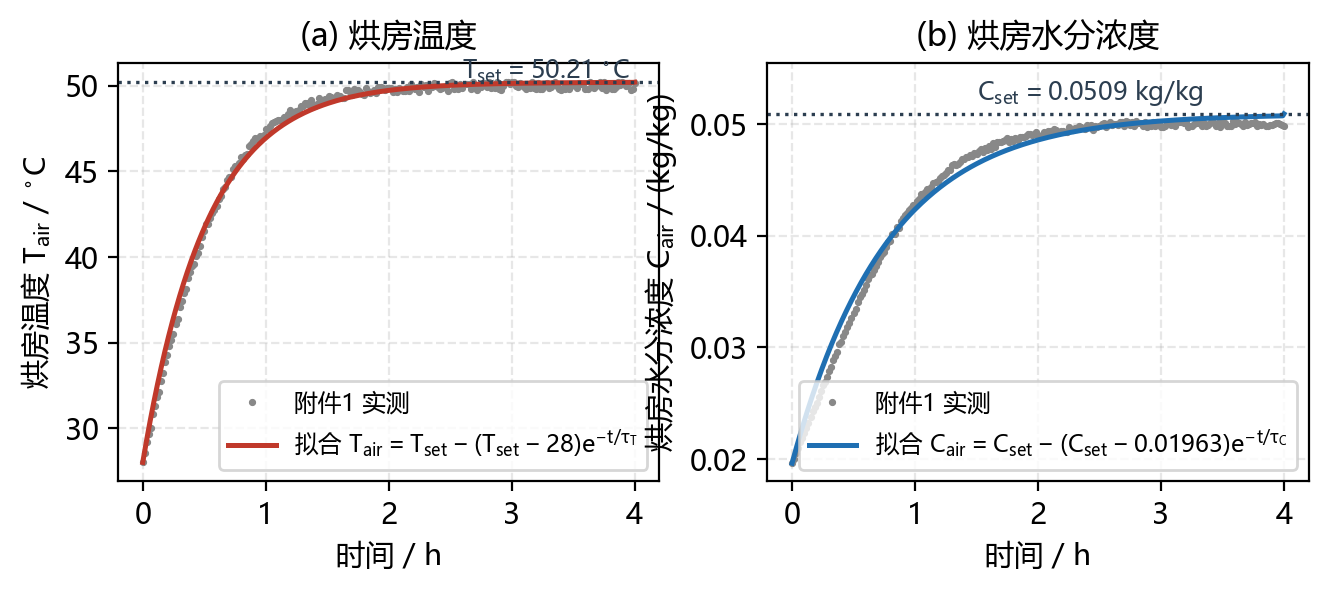
\includegraphics[width=0.84\textwidth]{figures/fig01_room_conditions.png}
  \caption{预热平衡阶段烘房环境参数及一阶惯性拟合}
  \label{fig:room}
\end{figure}

残差分析（图~\ref{fig:roomres}）显示：温度残差近似正态（偏度 $-0.37$、峰度
$2.94$），标准差 $0.334\,^\circ$C，处于仪表噪声量级；但滞后 1 阶自相关达
$0.83$，说明除随机噪声外还有\textbf{形式失配的系统性偏差}（最大绝对残差
$0.96\,^\circ$C）。该偏差\textbf{会}部分传递到解上：以原始实测序列作边界重算
（10.7 节表~\ref{tab:p1env}），表~\ref{tab:p1T} 各值最大降低 $0.52\,^\circ$C，
即拟合口径使温度表系统性偏高约 $0.5\,^\circ$C——定性结论（升温快于失水、
表 1 由表及里递减）不变，但这是问题 1 的主要误差来源，故两种口径一并列出。
湿度残差标准差 $8.0\times10^{-4}$ kg/kg（相对 $C_{set}$ 为 $1.6\%$），且只
影响水分浓度表的表面列（量级 $7\times10^{-4}$ kg/kg）。

\begin{figure}[htbp]
  \centering
  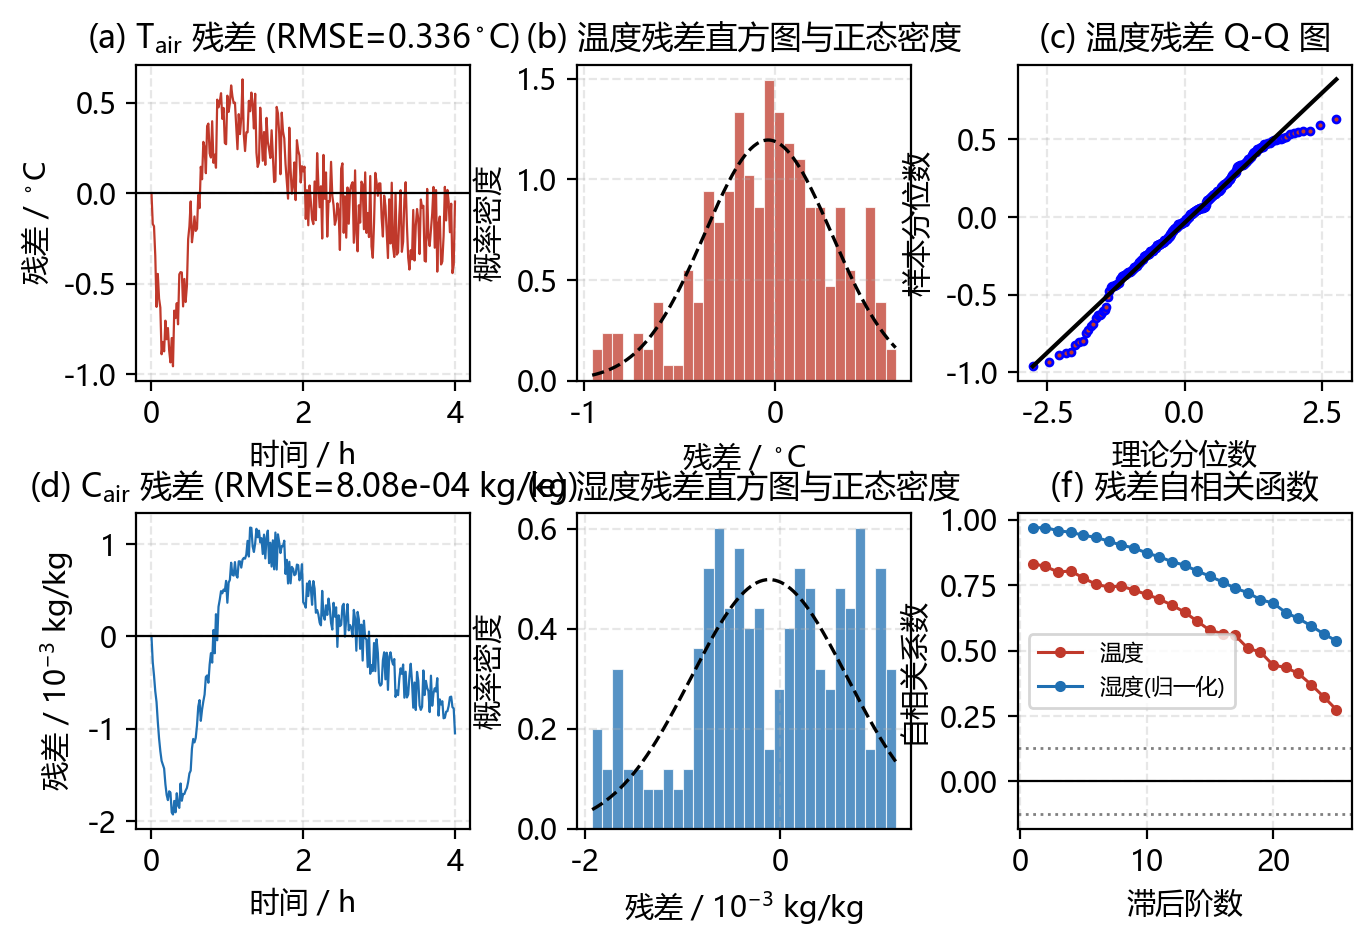
\includegraphics[width=0.84\textwidth]{figures/fig02_room_residuals.png}
  \caption{烘房环境拟合的残差诊断：(a)(d) 残差时序；(b)(e) 直方图与正态密度；
  (c) Q-Q 图；(f) 自相关函数}
  \label{fig:roomres}
\end{figure}

\textbf{物理合理性旁证}：把 $C_{air}$ 换算为相对湿度，$28\,^\circ$C 时
$w=0.01963$ kg/kg 对应 $p_v=3.10$ kPa、$\mathrm{RH}=82\%$；
$50\,^\circ$C 时 $w=0.0509$ kg/kg 对应 $p_v=7.67$ kPa、$\mathrm{RH}=62\%$
（$p_v=wp/(0.622+w)$，$p=101.325$ kPa，饱和压按 Hyland--Wexler 式）。
这分别落在「南方梅雨季环境空气」与「烘干房排湿工况」的合理范围内，
说明附件 1 的水分浓度确实是与药材含水率同一约定的\textbf{含湿量}，
从而式~\eqref{eq:robin} 中 $h_m(C_s-C_{air})$ 的量纲是自洽的。

\subsection{求解结果}

取 $N=1600$ 个控制体、$\Delta t=1$ s，按第 5 节的格式求解。
特征参数为 $\alpha=1.6886\times10^{-7}$ m$^2$/s、$Bi=1.3889$、
$\tau_T=2368.9$ s；$D(C_0)=4.9377\times10^{-9}$ m$^2$/s、$Bi_m=3.2404$、
$\tau_D=81010$ s。

表~\ref{tab:p1T} 与表~\ref{tab:p1C} 给出题目要求的温度与水分浓度，
完整结果（$1800$ s 内每 $1$ s、径向每 $0.1$ cm）见 \texttt{result1.xlsx}。

\begin{table}[htbp]
\centering
\caption{30 分钟内药材的温度（单位：$^\circ$C）}
\label{tab:p1T}
\footnotesize
\begin{tabular}{cccccc}
\toprule[1.5pt]
时间/s & $r=0$ & $r=0.5$ cm & $r=1.0$ cm & $r=1.5$ cm & $r=2.0$ cm \\
\midrule[1pt]
100  & 28.0001 & 28.0005 & 28.0054 & 28.0425 & 28.2219 \\
300  & 28.0500 & 28.0776 & 28.1857 & 28.4550 & 29.0261 \\
600  & 28.5456 & 28.6438 & 28.9618 & 29.5667 & 30.5576 \\
900  & 29.5568 & 29.7074 & 30.1740 & 30.9976 & 32.2359 \\
1200 & 30.9069 & 31.0882 & 31.6397 & 32.5824 & 33.9433 \\
1500 & 32.4397 & 32.6353 & 33.2248 & 34.2150 & 35.6117 \\
1800 & 34.0425 & 34.2411 & 34.8362 & 35.8249 & 37.1989 \\
\bottomrule[1.5pt]
\end{tabular}

\vspace{2pt}
{\footnotesize 注：本表以 6.1 节的一阶惯性拟合环境为边界。若直接以附件 1
实测序列插值为边界，本表各值将\textbf{系统性低} $0.41\!\sim\!0.52\,^\circ$C
（最大差值出现在 $t=1200$ s、$r=2.0$ cm 处），两套数值的完整对照见
10.7 节表~\ref{tab:p1env}。}
\end{table}

\begin{table}[htbp]
\centering
\caption{30 分钟内药材的水分浓度（单位：kg/kg）}
\label{tab:p1C}
\footnotesize
\begin{tabular}{cccccc}
\toprule[1.5pt]
时间/s & $r=0$ & $r=0.5$ cm & $r=1.0$ cm & $r=1.5$ cm & $r=2.0$ cm \\
\midrule[1pt]
100  & 2.5500 & 2.5500 & 2.5500 & 2.5500 & 2.2471 \\
300  & 2.5500 & 2.5500 & 2.5500 & 2.5492 & 2.0510 \\
600  & 2.5500 & 2.5500 & 2.5500 & 2.5353 & 1.8773 \\
900  & 2.5500 & 2.5500 & 2.5497 & 2.5046 & 1.7552 \\
1200 & 2.5500 & 2.5500 & 2.5482 & 2.4646 & 1.6592 \\
1500 & 2.5500 & 2.5499 & 2.5445 & 2.4207 & 1.5794 \\
1800 & 2.5500 & 2.5497 & 2.5383 & 2.3755 & 1.5109 \\
\bottomrule[1.5pt]
\end{tabular}
\end{table}

\begin{figure}[htbp]
  \centering
  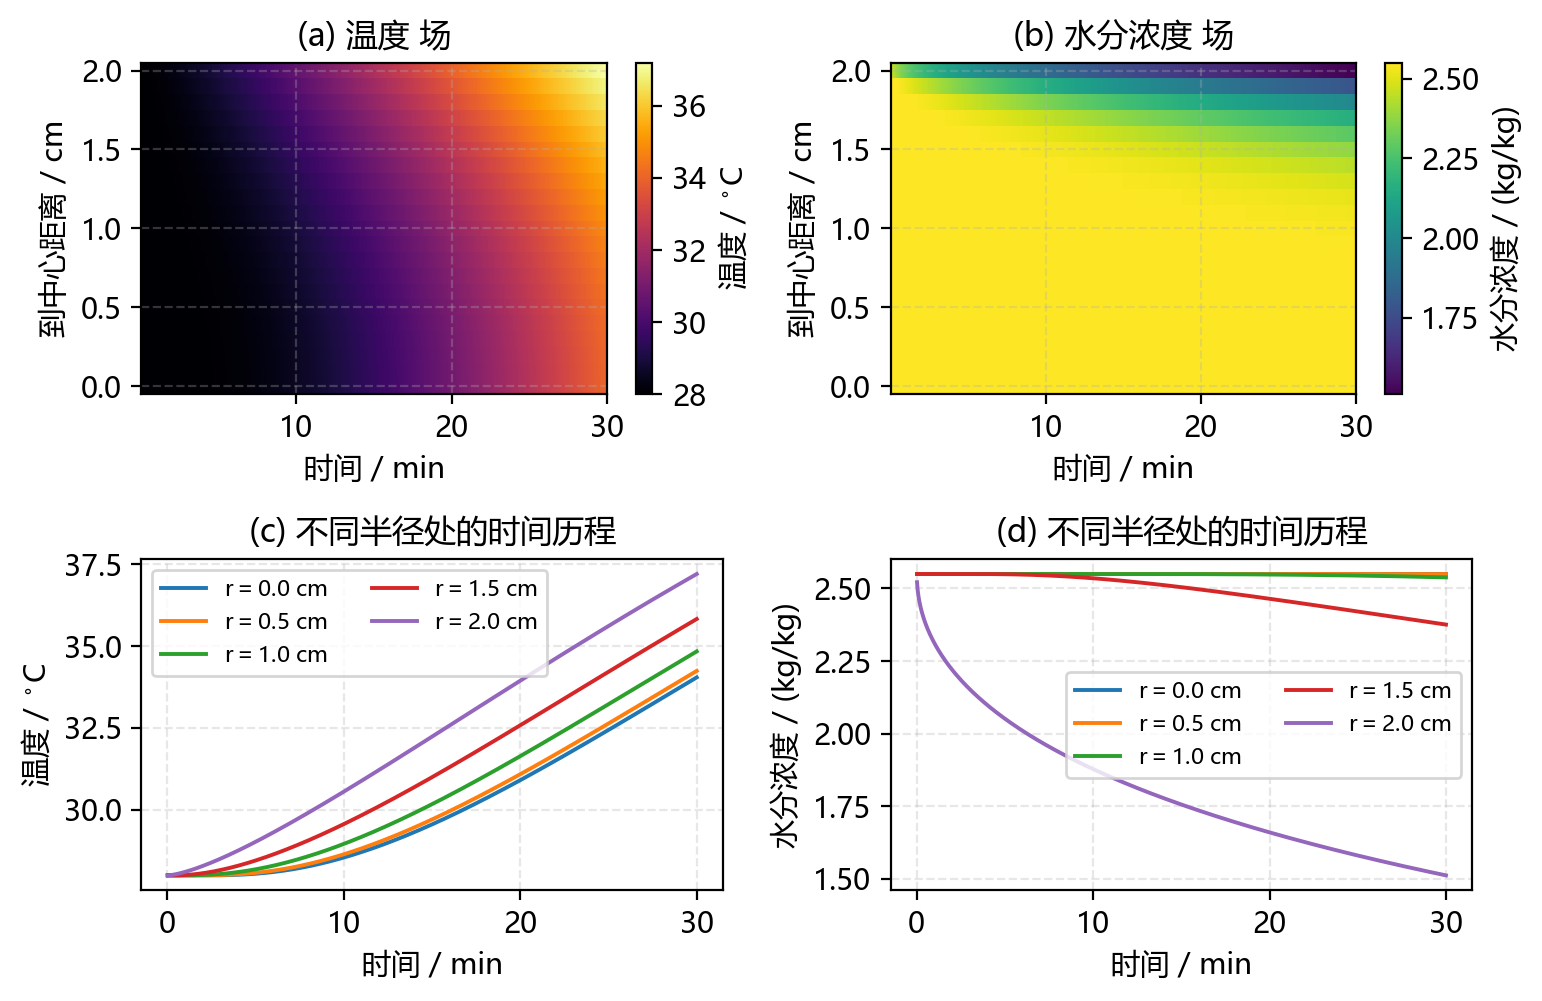
\includegraphics[width=0.84\textwidth]{figures/fig03_p1_fields.png}
  \caption{问题1：预热平衡阶段药材内部温度场与水分浓度场。(a)(b) 时空云图；
  (c)(d) 不同半径处的时间历程}
  \label{fig:p1fields}
\end{figure}

\subsection{结果分析}

\begin{figure}[htbp]
  \centering
  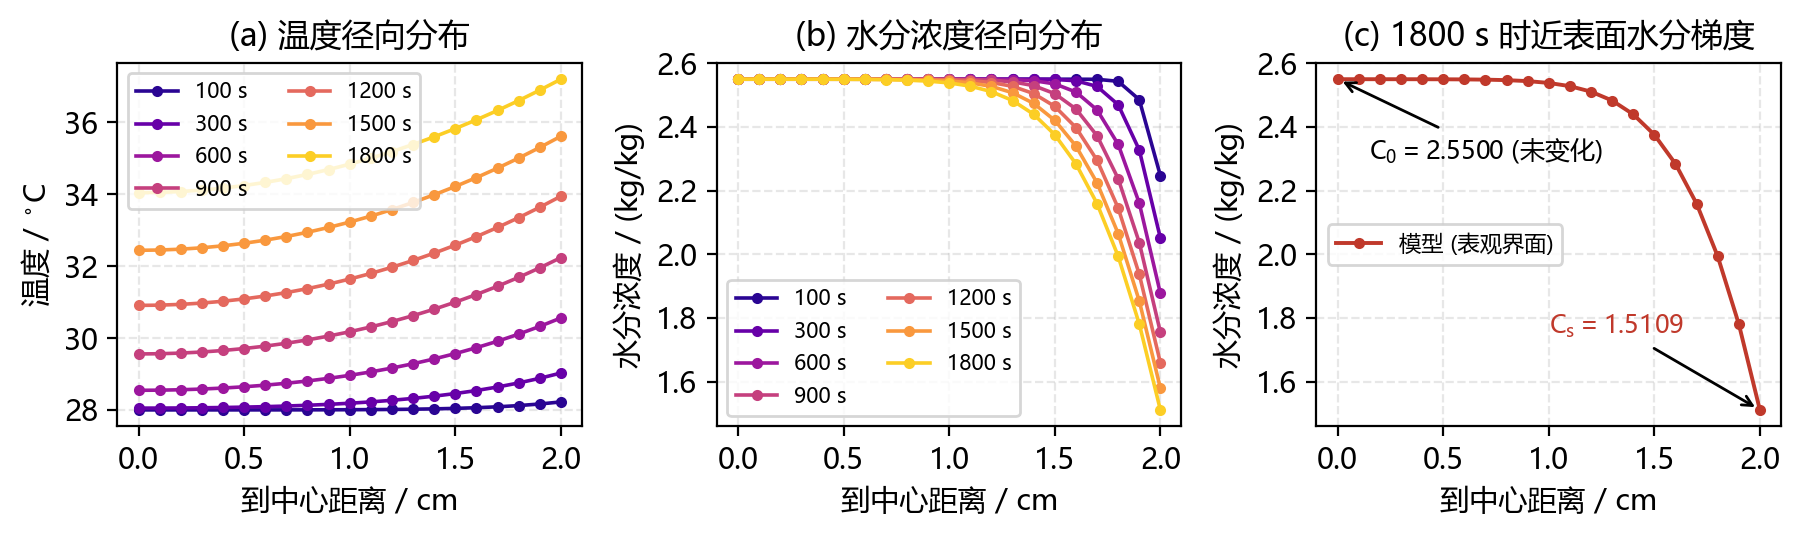
\includegraphics[width=0.84\textwidth]{figures/fig04_p1_profiles.png}
  \caption{问题1：温度与水分浓度的径向剖面演化，以及 1800 s 时的近表面水分梯度}
  \label{fig:p1prof}
\end{figure}

结果呈现清晰的\textbf{「热快质慢」}特征（图~\ref{fig:p1fields}、图~\ref{fig:p1prof}）：

\begin{enumerate}
  \item \textbf{温度场}：表面在 100 s 内即上升 $0.22\,^\circ$C，1800 s 时达到
  $37.1989\,^\circ$C；中心滞后明显，1800 s 时为 $34.0425\,^\circ$C，仅为表面
  与环境温差 $41.696-28=13.70\,^\circ$C 的 $44\%$。$Fo_T(1800\,\mathrm{s})=0.760$，
  与「预热阶段温度尚未完全平衡」的物理图像一致，也说明 30 分钟确实处在
  预热平衡阶段的中段。
  \item \textbf{水分场}：$r\le1.0$ cm 的三个位置在 1800 s 内几乎不变
  （中心 $2.5500$，1800 s 仍为 $2.5500$），而表面由 $2.55$ 降到 $1.5109$，
  降幅 $40.7\%$。这与 $Fo_D=0.0222$ 的数量级判断完全吻合：水分扩散的特征
  时间 $8.1\times10^4$ s 远大于 $1800$ s。
  \item \textbf{整体失水量}：截面平均含水（按面积加权）由 $2.5500$ 降到
  $2.2907$ kg/kg。按附录 2 的 $\rho=820$ kg/m$^3$ 与初始干基含水 $2.55$ 折算，
  干物质质量为 $72.57$ g、初始水量 $185.04$ g。数值解自 $t=1$ s 起采样，
  该时刻截面平均含水为 $2.5486$ kg/kg，由此算得 1800 s 内脱除水分
  $\mathbf{18.71}$ g，占初始水量的 $10.1\%$。若按模型内部约定把该失水速率
  换算为潜热负荷（水的汽化潜热取 $2383$ kJ/kg\cite{wagner2002}），
  1800 s 的平均表面潜热流为 $789$ W/m$^2$，而同期对流供热只有 $90$ W/m$^2$
  （$t=1800$ s 的瞬时值 $112$ W/m$^2$）：潜热负荷反而大一个量级，说明题给的
  $h_m$ 并非真实的 kg/(m$^2\cdot$s)；10.8 节据此论证该项无法由题面数据定量，
  故基准模型不计潜热。
\end{enumerate}

\textbf{模型的边界效应}：水分剖面的曲率在 $r>1.5$ cm 处急剧增大
（图~\ref{fig:p1prof}c），表面处一阶导约 $-270$ kg/kg/m（由 $r=1.9\to2.0$ cm
差分得到），与该时刻 Robin 条件给出的 $-h_m(C_s-C_{air})/D=-304$ kg/kg/m 在
$10\%$ 以内一致（差值来自差分的一阶截断误差）。这正是 $\exp(-0.89/C)$ 型
扩散系数导致的\textbf{表层快速失水}：表面含水率越低 $D$ 越小、剖面越陡，
形成正反馈——该非线性特征决定了必须用数值方法求解。

% =====================================================================
\section{问题二：整段烘干过程的模型建立与求解}

\subsection{两阶段工艺的刻画}

题目指出「预热平衡与恒温干燥阶段的参数有所不同」。由附件 1 可见烘房在 4 h
左右达到设定值并稳定（$t=4$ h 时 $T_{air}=49.99\,^\circ$C，为设定值的
$99.6\%$）。因此本文取

\begin{itemize}
  \item \textbf{预热平衡阶段} $0\le t\le14400$ s：环境按附件 1 的一阶惯性式变化；
  \item \textbf{恒温干燥阶段} $t>14400$ s：环境恒定为
  $T_{air}=T_{set}=50.212\,^\circ$C，$C_{air}=C_{set}=0.050908$ kg/kg。
\end{itemize}

恒温阶段取恒定含湿量是合理的：烘房必然持续排湿，否则由药材 4 h 内蒸发的水量
（约 95 g）反推，密闭腔体的含湿量增量会远超饱和值。取附件 1 拟合式的终值为
稳态值，与实测末段均值 $50.02\,^\circ$C、$0.0500$ kg/kg 相差在
$0.2\,^\circ$C 与 $10^{-3}$ kg/kg 以内。
物性改用附录 3 的关系式，方程与边界条件同式~\eqref{eq:heat}--\eqref{eq:robin}。

\subsection{求解结果}

表~\ref{tab:p2T}、表~\ref{tab:p2C} 给出 3 h 内每 $0.5$ h 的结果，
图~\ref{fig:p23fields} 给出整段过程的时空场。

\begin{table}[htbp]
\centering
\caption{3 小时内药材的温度（单位：$^\circ$C）}
\label{tab:p2T}
\footnotesize
\begin{tabular}{cccccc}
\toprule[1.5pt]
时间/h & $r=0$ & $r=0.5$ cm & $r=1.0$ cm & $r=1.5$ cm & $r=2.0$ cm \\
\midrule[1pt]
0.5 & 32.5656 & 32.7627 & 33.3570 & 34.3573 & 35.7831 \\
1.0 & 40.4220 & 40.5818 & 41.0548 & 41.8230 & 42.8629 \\
1.5 & 45.5851 & 45.6719 & 45.9272 & 46.3366 & 46.8815 \\
2.0 & 48.2253 & 48.2650 & 48.3814 & 48.5675 & 48.8138 \\
2.5 & 49.4129 & 49.4293 & 49.4775 & 49.5546 & 49.6565 \\
3.0 & 49.9051 & 49.9115 & 49.9302 & 49.9602 & 49.9999 \\
\bottomrule[1.5pt]
\end{tabular}
\end{table}

\begin{table}[htbp]
\centering
\caption{3 小时内药材的水分浓度（单位：kg/kg）}
\label{tab:p2C}
\footnotesize
\begin{tabular}{cccccc}
\toprule[1.5pt]
时间/h & $r=0$ & $r=0.5$ cm & $r=1.0$ cm & $r=1.5$ cm & $r=2.0$ cm \\
\midrule[1pt]
0.5 & 2.5499 & 2.5488 & 2.5247 & 2.3237 & 1.6538 \\
1.0 & 2.5248 & 2.4935 & 2.3562 & 2.0227 & 1.4709 \\
1.5 & 2.3860 & 2.3258 & 2.1350 & 1.8020 & 1.3444 \\
2.0 & 2.1731 & 2.1105 & 1.9250 & 1.6256 & 1.2282 \\
2.5 & 1.9589 & 1.9025 & 1.7369 & 1.4716 & 1.1157 \\
3.0 & 1.7673 & 1.7174 & 1.5705 & 1.3332 & 1.0083 \\
\bottomrule[1.5pt]
\end{tabular}
\end{table}

\begin{figure}[htbp]
  \centering
  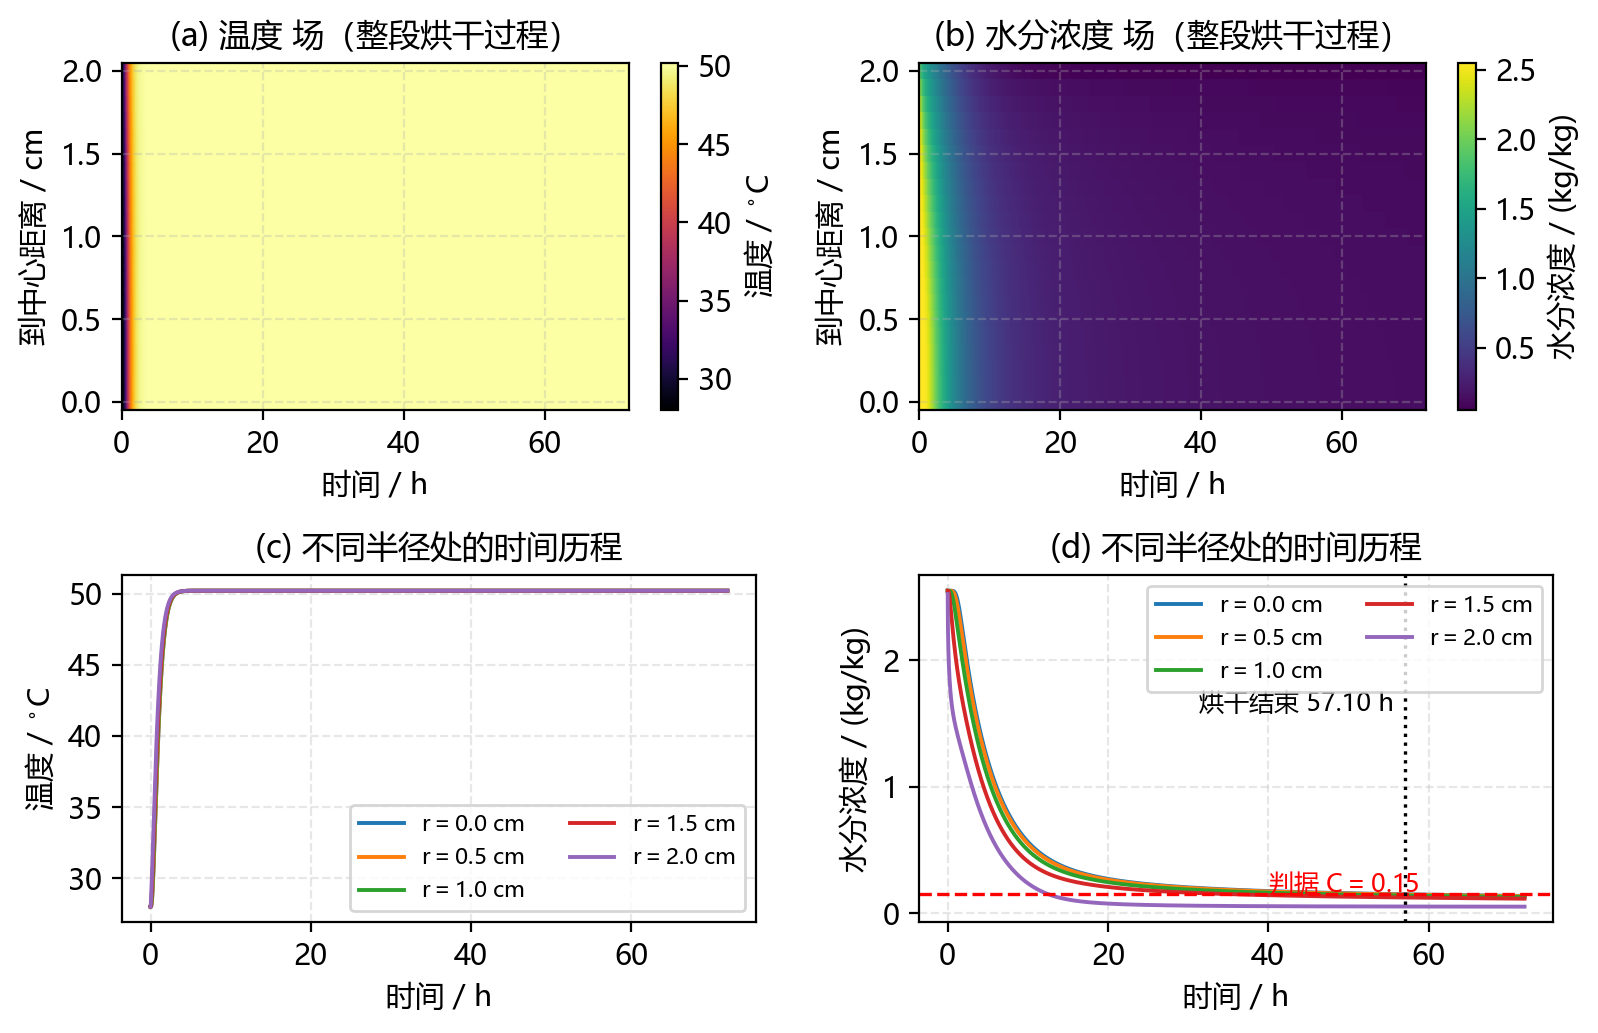
\includegraphics[width=0.84\textwidth]{figures/fig07_p23_fields.png}
  \caption{问题2：整段烘干过程的温度场与水分浓度场}
  \label{fig:p23fields}
\end{figure}

\subsection{结果分析}

\begin{enumerate}
    \item \textbf{温度在 2 h 内基本完成平衡}。由表~\ref{tab:p2T}，1 h 时中心
  $40.42\,^\circ$C、2 h 时 $48.23\,^\circ$C、3 h 时 $49.91\,^\circ$C，
  与环境温差仅 $0.3\,^\circ$C；径向差也从 1 h 的 $2.44\,^\circ$C 收缩到
  3 h 的 $0.09\,^\circ$C。这说明\textbf{恒温干燥阶段药材可近似视为等温体}，
  与 $\mathrm{Le}=0.093$（热扩散远快于水分扩散）的无量纲判断一致。
  \item \textbf{水分剖面由「平缓」转为「陡峭」}（图~\ref{fig:p8}）。3 h 时
  中心 $1.7673$、$r=1.5$ cm 处 $1.3332$、表面 $1.0083$ kg/kg，
  剖面斜率随 $r$ 单调增大。这是 $D$ 随 $C$ 指数下降的直接后果：表面先失水，
  表面层的 $D$ 随之下降，形成「干壳」，内部的水分必须穿过阻力越来越大的
  外壳才能迁出。
  \item \textbf{失水速率呈现典型的降速特征}（图~\ref{fig:p9}b）。表面传质通量
  $h_m(C_s-C_{air})$ 由 6 h 的 $3.87\times10^{-7}$ 单调降到 72 h 的
  $1.4\times10^{-9}$（模型单位），跨越两个多数量级，与「恒速期—降速期」的
  干燥理论一致，而本模型中没有独立设定恒速期，它\textbf{自动涌现}于
  $D(C,T)$ 的经验式。
\end{enumerate}

\begin{figure}[htbp]
  \centering
  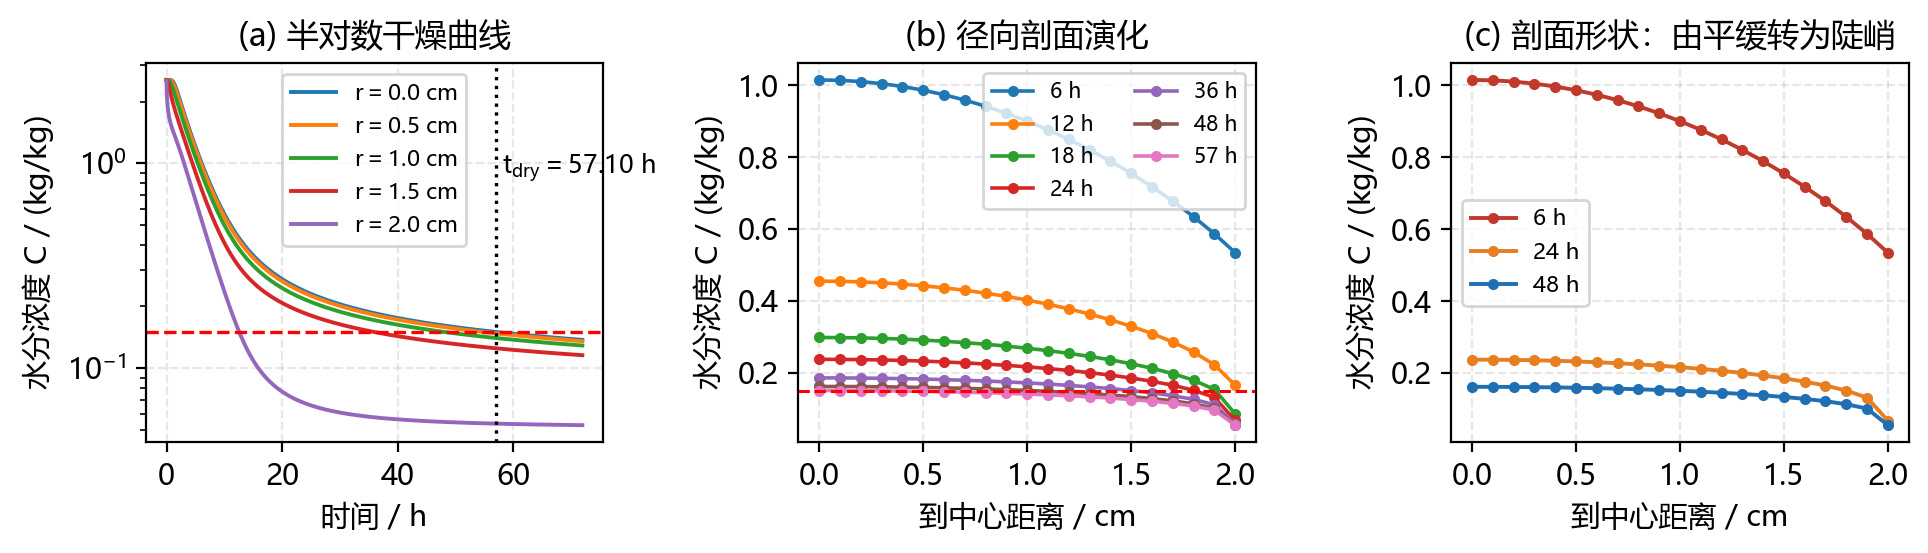
\includegraphics[width=0.84\textwidth]{figures/fig08_p23_curves.png}
  \caption{问题2--3：半对数干燥曲线、径向剖面演化与剖面形状变化}
  \label{fig:p8}
\end{figure}

\begin{figure}[htbp]
  \centering
  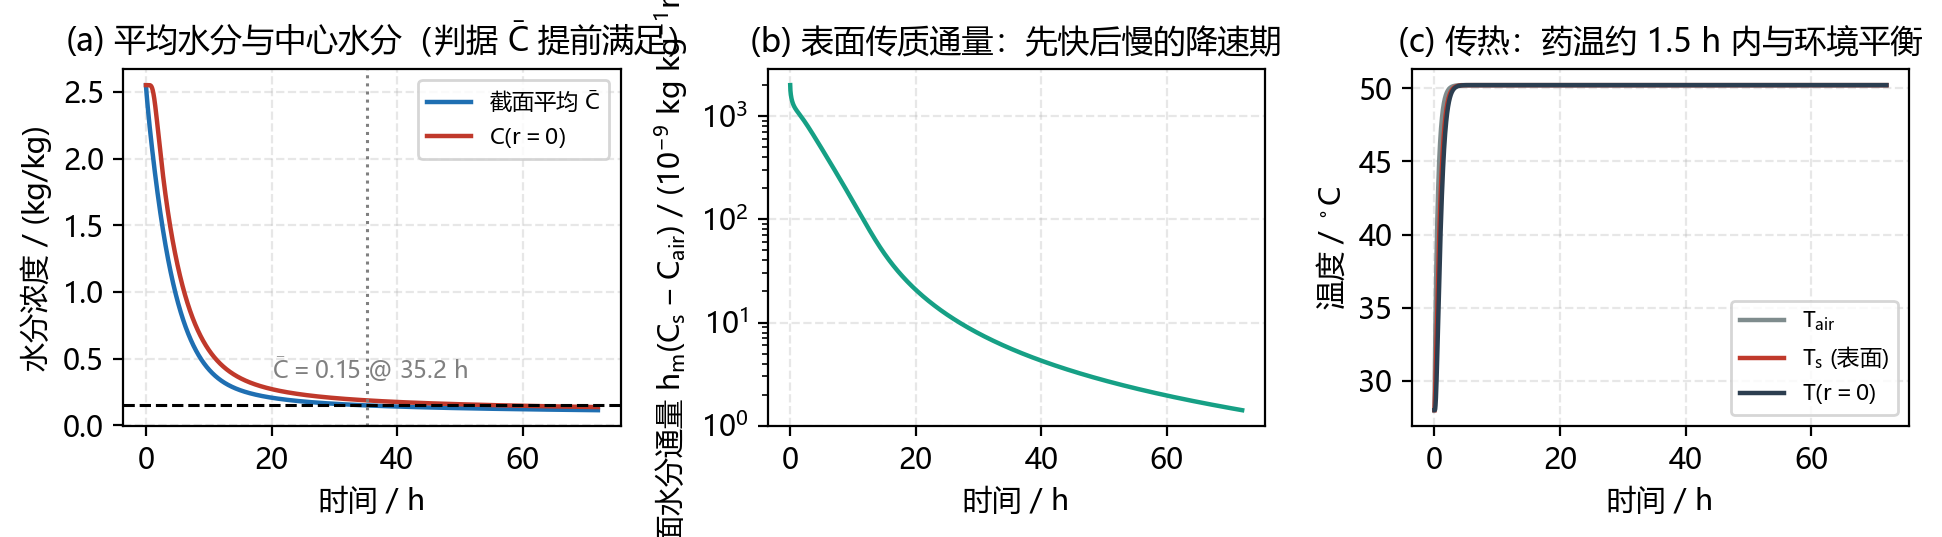
\includegraphics[width=0.84\textwidth]{figures/fig09_p23_flux.png}
  \caption{问题2--3：平均水分与中心水分、表面传质通量、传热弛豫过程}
  \label{fig:p9}
\end{figure}

% =====================================================================
\section{问题三：烘干时间的确定}

\subsection{判据的数学表述与关键判断}

题目要求「药材各处的水分浓度应低于 $0.15$ kg/kg」，即

\begin{equation}
t_{dry}=\min\left\{t>0\ :\ \max_{0\le r\le R_0}C(r,t)<0.15\right\}.
\label{eq:criterion}
\end{equation}

\textbf{关键判断}：圆柱几何下中心点的扩散路径最长，因此必然是最后干燥的
位置。本文不预设这一点，而是逐时刻检验，且\textbf{最大值取在全部
$N+1=1601$ 个节点}上，而不是只在 $21$ 个输出位置上取最大（后者在原理上可能
漏掉真正的极值点）。判据须表述为 $C_{\max}(t)-C(0,t)\le
10^{-12}C_{\max}$；至于「$\arg\max$ 的索引是否为 $0$」，在剖面仍均匀到
舍入精度的初始阶段只是大量节点并列的结果，不承载物理信息。检验结果
（\texttt{p23\_summary.txt}、\texttt{p4\_summary.txt}）：问题 2--3 与问题 4 的
\textbf{全部输出时刻}均满足该判据（问题 4 的最大相对超出量仅
$6.1\times10^{-15}$，纯属舍入），\textbf{数据证实了该判断}；问题 4 的
$259200$ 个时刻中有 $256746$ 个 $\arg\max$ 落在 $\xi=0$，其余 $2454$ 个
集中在最初阶段。
式~\eqref{eq:criterion} 中取严格小于号，因此 $t_{dry}$ 由 $C(0,t)$ 首次
下穿 $0.15$ 的时刻给出，本文在 $C(0,t)$ 上做线性插值精确求交。

\subsection{结果}

\begin{table}[htbp]
\centering
\caption{药材烘干过程的水分浓度（单位：kg/kg）}
\label{tab:p3}
\footnotesize
\begin{tabular}{cccccc}
\toprule[1.5pt]
时间/h & $r=0$ & $r=0.5$ cm & $r=1.0$ cm & $r=1.5$ cm & $r=2.0$ cm \\
\midrule[1pt]
6  & 1.0149 & 0.9863 & 0.9003 & 0.7548 & 0.5343 \\
12 & 0.4546 & 0.4417 & 0.4019 & 0.3291 & 0.1651 \\
18 & 0.2978 & 0.2905 & 0.2678 & 0.2247 & 0.0853 \\
24 & 0.2370 & 0.2320 & 0.2160 & 0.1850 & 0.0673 \\
30 & 0.2052 & 0.2012 & 0.1886 & 0.1636 & 0.0607 \\
36 & 0.1853 & 0.1820 & 0.1713 & 0.1500 & 0.0575 \\
42 & 0.1716 & 0.1686 & 0.1593 & 0.1404 & 0.0557 \\
48 & 0.1614 & 0.1588 & 0.1503 & 0.1331 & 0.0546 \\
54 & 0.1535 & 0.1510 & 0.1433 & 0.1274 & 0.0539 \\
\textbf{烘干结束（$N=1600$ 直接值 $57.0983$ h）} & \textbf{0.1500} & 0.1477 & 0.1402 & 0.1249 & 0.0536 \\
\bottomrule[1.5pt]
\end{tabular}
\end{table}

\begin{equation}
\boxed{\ t_{dry}=205559\ \mathrm{s}=57.10\ \mathrm{h}=2.379\ \mathrm{d}\ }
\end{equation}

上表末行是 $N=1600$ 网格上的\textbf{直接计算值} $205553.8$ s $=57.0983$ h；
式中的 $205559$ s $=57.100$ h 是该序列经 Richardson 外推的\textbf{收敛值}
（10.2 节），两者相差 $5.5$ s（$0.0027\%$），正文一律以后者为准。此时
$C(0,t_{dry})=0.1500$（判据恰好满足），表面 $C_s=0.0536$ kg/kg；按
$2\int_0^1C\xi\,\mathrm{d}\xi$ 的梯形积分（最外层控制体只有半个单元厚，
面积加权时表面点权重取半）得截面平均含水 $0.1232$ kg/kg。

\subsection{结果分析}

\begin{figure}[htbp]
  \centering
  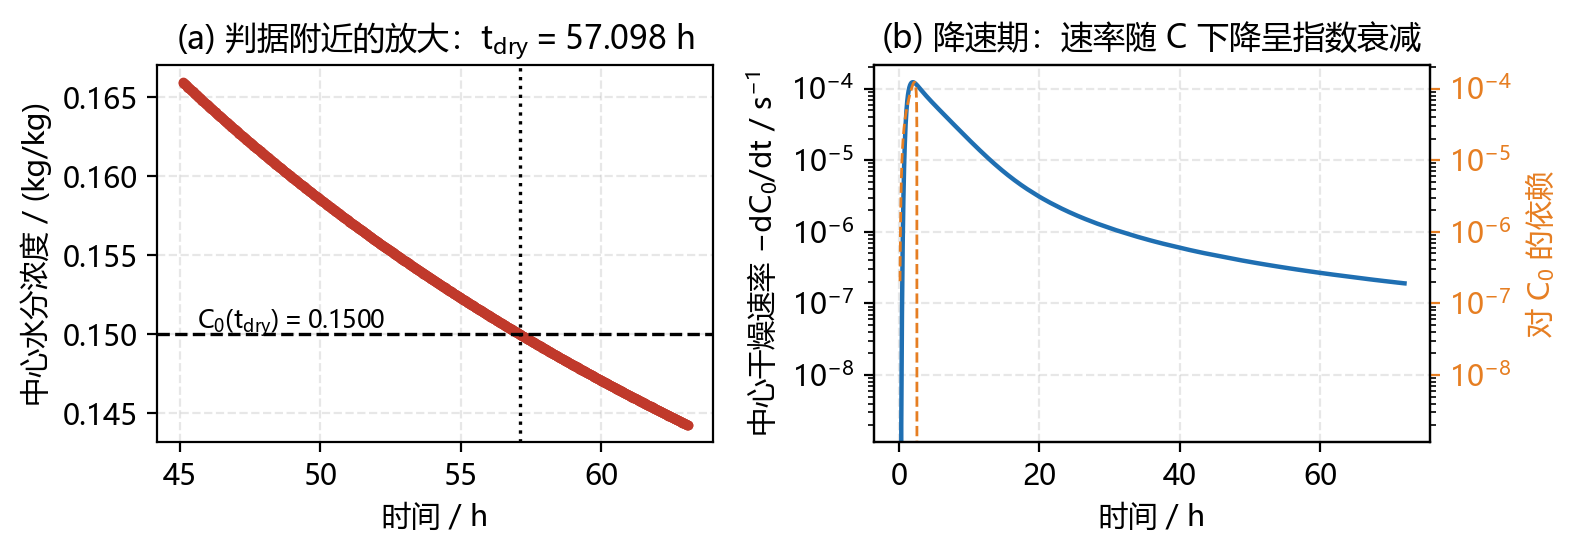
\includegraphics[width=0.84\textwidth]{figures/fig10_p23_zoom.png}
  \caption{烘干终点的精细刻画与降速干燥特征}
  \label{fig:p10}
\end{figure}

\begin{enumerate}
  \item \textbf{与题目经验一致}。题目称「烘干过程一般持续 2--3 天」，
  本文模型独立计算出 $2.379$ 天，落在区间内且不贴边，说明模型对整体
  时间尺度的刻画是可信的。
  \item \textbf{判据的「迟滞」效应}（图~\ref{fig:p10}a）。截面平均含水在
  $35.17$ h 就已降到 $0.15$ kg/kg，但中心要到 $57.10$ h 才达标，滞后 $21.9$ h。
  这说明\textbf{以平均值判定干燥终点会严重低估所需时间}（低估 $38\%$），
  必须采用逐点判据。这一结论对工艺控制有直接意义。
  \item \textbf{降速期的定量特征}（图~\ref{fig:p10}b）。中心干燥速率
  $-\mathrm{d}C_0/\mathrm{d}t$ 本身呈\textbf{指数衰减}：用相邻表列值作
  中心差分，$\ln(-\dot C_0)$ 对 $t$ 的斜率在 $30\!\sim\!54$ h 约为
  $-0.051$ h$^{-1}$、在 $36\!\sim\!54$ h 约为 $-0.046$ h$^{-1}$，对应
  速率衰减的特征时间 $20\!\sim\!22$ h；同一区间内 $C_0$ 自身的对数斜率
  只有 $-0.011$ h$^{-1}$，速率衰减明显快于浓度衰减，这正是降速干燥期的标志。
\end{enumerate}

% =====================================================================
\section{问题四：考虑尺寸收缩的模型建立与求解}

\subsection{收缩数据的处理}

附件 2 给出 $0\sim259200$ s 内每 $1800$ s 一次的药材半径，共 145 个点。
数据单调不增：由 $R(0)=2.000$ cm 迅速下降到 $R(241200\,\mathrm{s})=1.198$ cm，
之后保持不变，半径比 $R/R_0=0.599$。由此得两个口径下的收缩幅度：按本文的
无限长圆柱假定（只径向收缩），单位长度的体积（横截面积）比为
$(R/R_0)^2=0.359$；若按各向同性收缩（长径同比例减小，10.6 节的对照口径），
体积比为 $(R/R_0)^3=0.215$。收缩建模的常见做法与本文一致，即用实测或拟合的
$R(t)$ 直接驱动几何\cite{mayor2004,kowalski1996}。
对比两种描述（图~\ref{fig:p11}）：单指数拟合
$R=R_\infty+(R_0-R_\infty)e^{-t/\tau_R}$（$R_0$ 固定为实测初值 $2.000$ cm）
给出 $R_\infty=1.2022$ cm、$\tau_R=3.79$ h、RMSE $=8.1\times10^{-3}$ cm
（放开 $R_0$ 可把 RMSE 降到 $6.2\times10^{-3}$ cm，但拟合出的
$R_0=1.960$ cm 与附件 2 明载的 $2.000$ cm 矛盾，故不采用）；分段线性插值则在
所有实测点上精确通过。

本文\textbf{采用分段线性插值}作为主模型（$dR/dt$ 用中心差分），并在灵敏度
分析中用指数拟合做对照（两者 $t_{dry}$ 相差 $0.09$ h）。附件 2 的收缩
\textbf{前期最快}：$|\mathrm{d}R/\mathrm{d}t|$ 在 $t=0$ 处最大
（$7.06\times10^{-7}$ m/s），$t=0.5$ h 时 $5.72\times10^{-7}$ m/s、
$t=12$ h 时 $2.5\times10^{-8}$ m/s；$90\%$ 的收缩在前 $10$ h 内完成。
逐段差分得到的 $|\mathrm{d}R/\mathrm{d}t|$ 序列中有十余处幅度不超过峰值
$2\%$ 的局部回升（最大 $1.6\%$），属测量噪声；$R(t)$ 本身严格单调不增。
\begin{figure}[htbp]
  \centering
  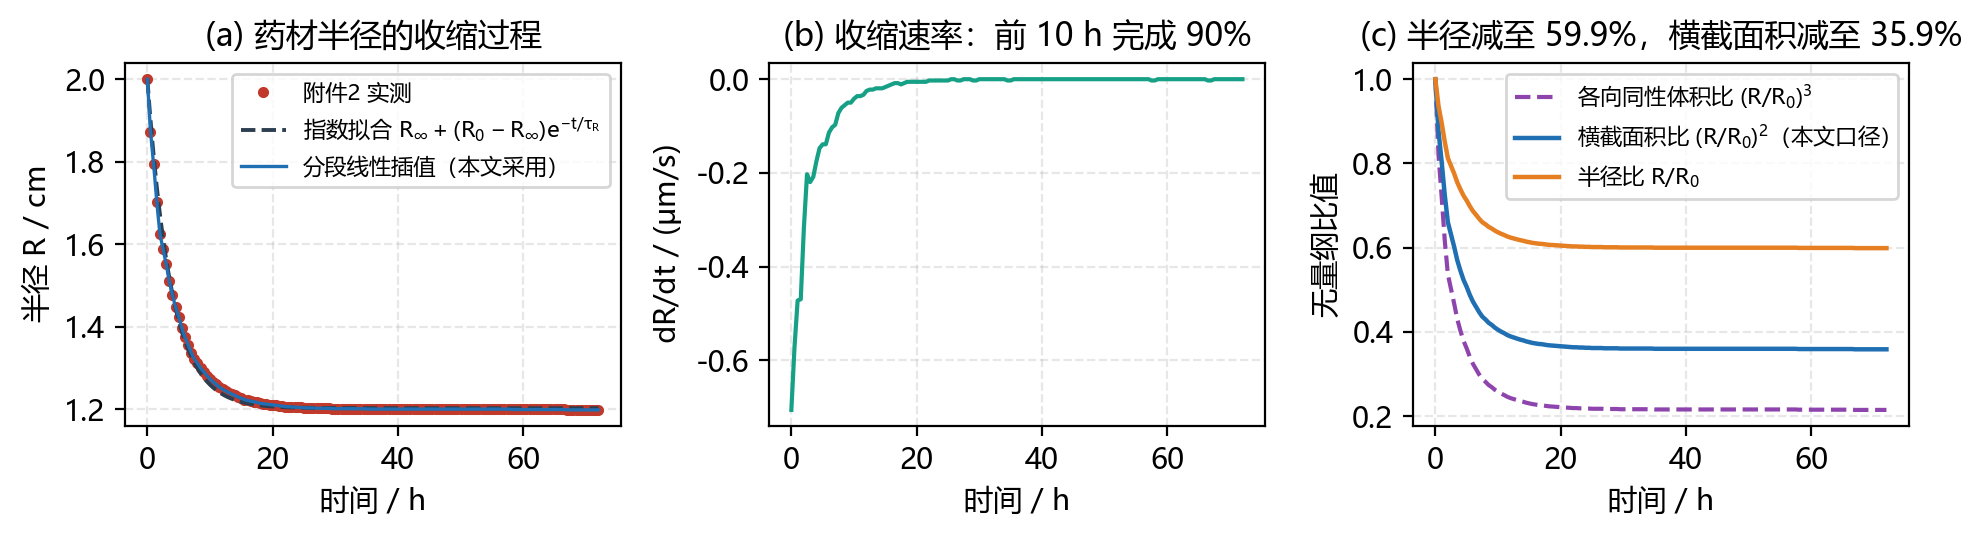
\includegraphics[width=0.84\textwidth]{figures/fig11_p4_radius.png}
  \caption{问题4：附件 2 给出的药材半径历史、收缩速率与无量纲收缩比}
  \label{fig:p11}
\end{figure}

\subsection{模型与求解}

模型即 5.5 节的式~\eqref{eq:shrink} 与式~\eqref{eq:heat-shrink}，
物性取附录 4。烘房环境与问题 2--3 相同（同一台设备）。

\textbf{输出约定}。题目表 6 要求给出「到药材中心距离每隔 $0.5$ cm」的水分
浓度，末列为「药材表面」。这里必须区分两个坐标：求解器工作在\textbf{物质坐标}
$\xi=r/R(t)$ 上，而表格列名是\textbf{当前物理距离} $r$，由 $r=\xi R(t)$
联系，同一列在不同时刻对应不同材料点。本文对每个输出时刻在 $\xi=r_j/R(t_i)$
处采样，得到当前物理距离 $r_j$ 处的水分浓度；$r_j>R(t_i)$（如 $r=1.5$ cm 在
$t>3.67$ h 后）留空，末列给出当前表面值 $C(R(t_i),t_i)$；实现上即采样位置随
输出时刻变化。若误在固定 $\xi$ 剖面上插值，会把 $\xi$ 处的值标成 $r$ 处的值
（9.4 节量化了该误差）。物质坐标下的完整剖面（$21$ 列无空缺）另存为
\texttt{result4\_material\_coord.xlsx}。

\subsection{结果}

\begin{table}[htbp]
\centering
\caption{药材烘干过程的水分浓度（问题4，含收缩；列名为当前物理距离，单位：kg/kg）}
\label{tab:p4}
\footnotesize
\begin{tabular}{ccccccc}
\toprule[1.5pt]
时间/h & $R(t)$/cm & $r=0$ & $r=0.5$ cm & $r=1.0$ cm & $r=1.5$ cm & 药材表面 \\
\midrule[1pt]
6  & 1.374 & 1.7157 & 1.5345 & 1.0215 & --- & 0.4228 \\
12 & 1.248 & 0.7335 & 0.6512 & 0.4069 & --- & 0.1677 \\
18 & 1.214 & 0.4062 & 0.3665 & 0.2388 & --- & 0.0899 \\
24 & 1.204 & 0.2835 & 0.2596 & 0.1783 & --- & 0.0681 \\
30 & 1.201 & 0.2251 & 0.2083 & 0.1488 & --- & 0.0603 \\
36 & 1.200 & 0.1919 & 0.1788 & 0.1313 & --- & 0.0568 \\
42 & 1.200 & 0.1705 & 0.1597 & 0.1196 & --- & 0.0550 \\
48 & 1.200 & 0.1555 & 0.1462 & 0.1113 & --- & 0.0539 \\
\textbf{烘干结束 $50.7678$ h} & \textbf{1.200} & \textbf{0.1500} & 0.1413 & 0.1081 & --- & 0.0535 \\
\bottomrule[1.5pt]
\end{tabular}

\vspace{2pt}
{\footnotesize ``---''表示该物理距离已位于收缩后的药材之外（$r_j>R(t)$），
位置不存在故不填数值。$r=1.5$ cm 列自 $t>3.67$ h 起即为空
（$R(t)$ 与 $1.5$ cm 的交点，见 9.2 节）。
数据取自 \texttt{data/result4.xlsx}；完整无空缺的物质坐标剖面见
\texttt{result4\_material\_coord.xlsx}。}
\end{table}

\begin{equation}
\boxed{\ t_{dry}=182765\ \mathrm{s}=50.77\ \mathrm{h}=2.115\ \mathrm{d}\ }
\end{equation}

\begin{figure}[htbp]
  \centering
  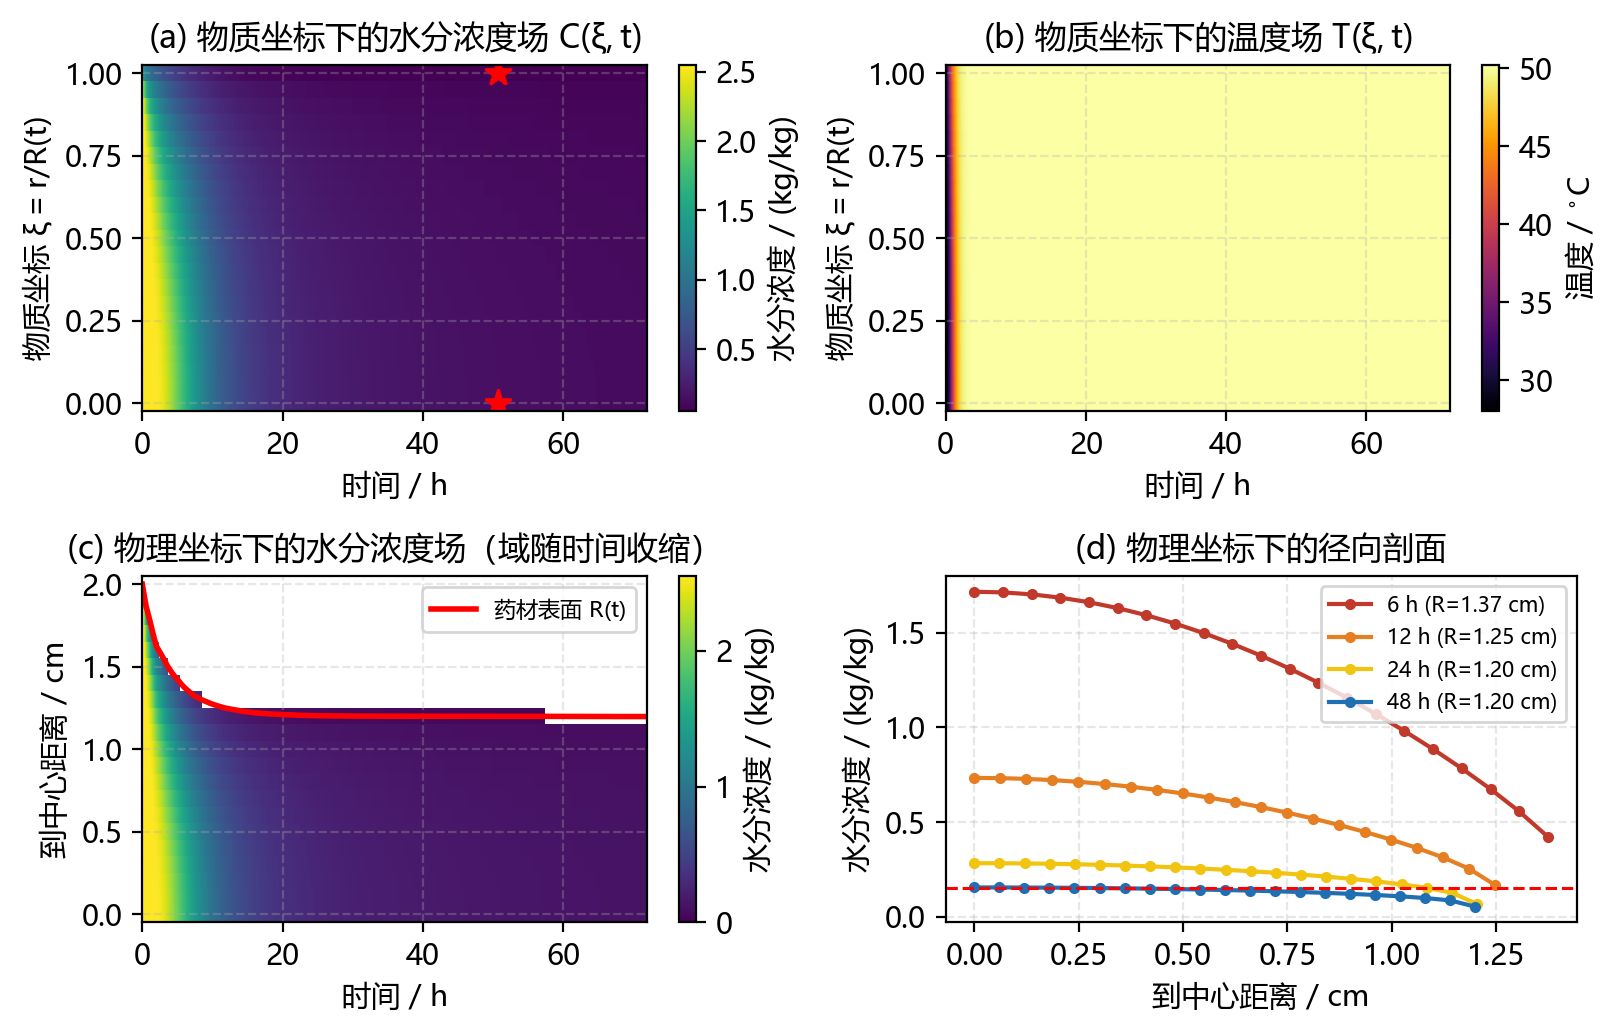
\includegraphics[width=0.84\textwidth]{figures/fig12_p4_fields.png}
  \caption{问题4：考虑收缩后的水分浓度场。(a)(b) 物质坐标下的水分与温度场
  ——(b) 中温度在约 $2$ h 后即与环境一致（全场极差 $<0.1\,^\circ$C），
  故整幅趋于同色，这本身就是 7.3 节「恒温阶段可近似视为等温体」的图示证据；
  (c) 物理坐标下的水分浓度场，纵轴为当前物理距离、红色曲线为收缩中的表面
  $R(t)$，$r>R(t)$ 的区域留白；(d) 物理坐标下的径向剖面}
  \label{fig:p12}
\end{figure}

\subsection{结果分析}

\begin{enumerate}
    \item \textbf{收缩显著缩短干燥时间}。与「物性取附录 4 但半径固定为
  $2$ cm」的对照算例相比，不收缩时 $t_{dry}=128.90$ h（$5.37$ 天），收缩时为
  $50.77$ h，\textbf{缩短 $60.6\%$}（即忽略收缩会把烘干时间高估 $2.5$ 倍）。
  机理是双重的：半径由 $2.000$ 减到 $1.198$ cm 使扩散长度平方降至 $35.9\%$，
  同时表面面积减小使总失水速率下降，但前者占主导——这是必须建模的效应。
  \item \textbf{收缩完成后进入准等径干燥}（图~\ref{fig:p12}）。$t>24$ h 后
  $R\approx1.20$ cm 基本不变，此后过程退化为半径 $1.2$ cm 的固定域问题，
  在物质坐标云图（图~\ref{fig:p12}a）上表现为 $C(\xi,t)$ 的等值线在后期
  趋于垂直。
    \item \textbf{物理坐标与物质坐标的差异}（图~\ref{fig:p12}c,d）。在物理坐标下
  同一位置在不同时刻对应不同材料点：$r=1.0$ cm 处 $6$ h 时对应
  $\xi=0.728$（已是当时的表层）、$48$ h 时对应 $\xi=0.833$。若把固定 $\xi$
  剖面直接当作物理距离填表，$6$ h 时 $r=1.0$ cm 处会给出 $C(\xi=0.5)=1.3782$，
  而真值为 $1.0215$（$+35\%$），$12$ h 时误差达 $+49\%$（$0.6059$ 对
  $0.4069$）；「$r=1.5$ cm 列在 $3.67$ h 后为空」也是同一映射关系的产物。
\item \textbf{与问题 3 的对比}（图~\ref{fig:p13}）。两条中心干燥曲线在
  $t<10$ h 时几乎重合，之后收缩算例明显更快；两者的表面浓度曲线在整个
  过程中都紧贴环境平衡值（$C_{air}=0.0509$），差值在 $0.003$ kg/kg 以内，
  说明表面长期处于准平衡状态。
\end{enumerate}

\begin{figure}[htbp]
  \centering
  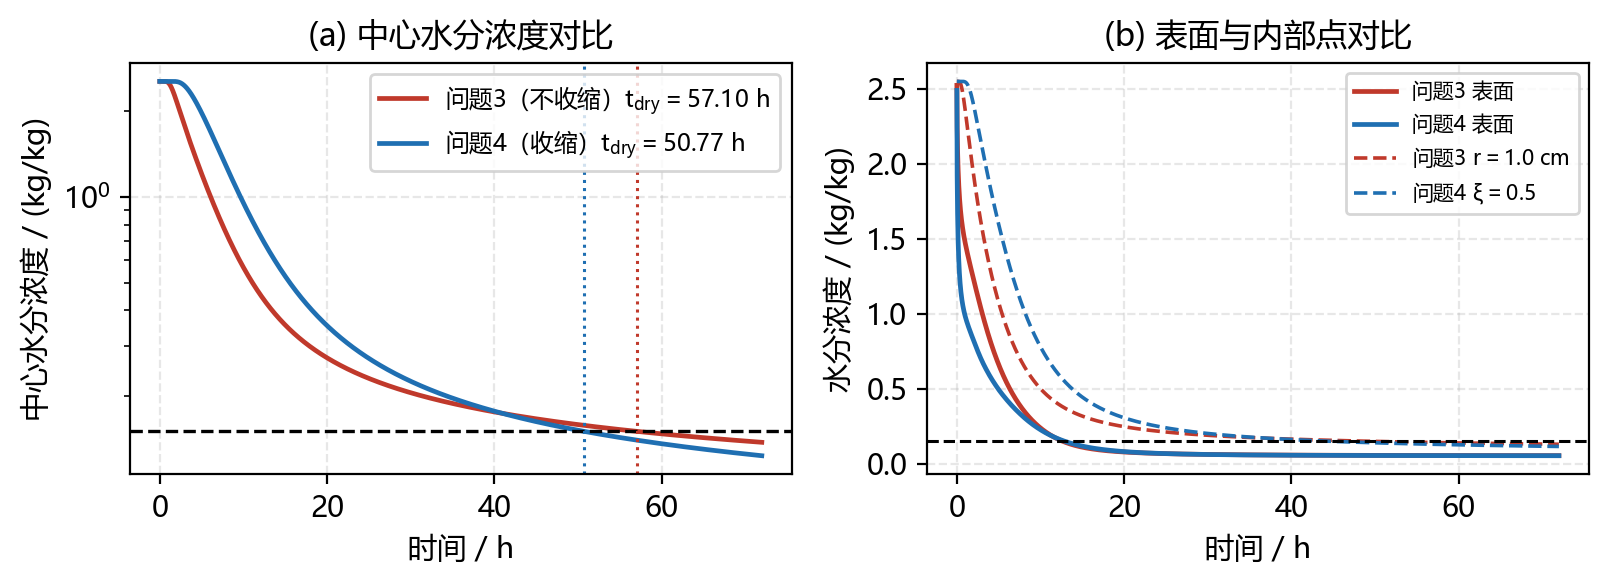
\includegraphics[width=0.84\textwidth]{figures/fig13_p3_vs_p4.png}
  \caption{收缩对干燥过程的影响：问题3 与问题4 结果对比}
  \label{fig:p13}
\end{figure}

% =====================================================================
\section{模型检验与灵敏度分析}

本章按「解析验证 $\to$ 离散收敛性 $\to$ 守恒性 $\to$ 多方法互证 $\to$
外部数据校验 $\to$ 参数灵敏度 $\to$ 不确定度汇总」的顺序逐层检验。

\subsection{解析解验证（常物性、恒环境）}

当物性为常数、环境恒定时，式~\eqref{eq:heat}--\eqref{eq:robin} 存在 Bessel
级数解析解\cite{carslaw1959,crank1975}：

\begin{equation}
\frac{\phi-\phi_\infty}{\phi_0-\phi_\infty}
=\sum_{n=1}^{\infty}A_nJ_0\!\left(\mu_n\frac{r}{R_0}\right)
\exp\!\left(-\mu_n^2\frac{at}{R_0^2}\right),\qquad
A_n=\frac{2J_1(\mu_n)}{\mu_n\left[J_0^2(\mu_n)+J_1^2(\mu_n)\right]},
\end{equation}

其中 $\mu_n$ 是 $\mu J_1(\mu)=Bi\,J_0(\mu)$ 的正根，$a$ 与 $Bi$ 分别取
（热/质）对应的系数。取 $T_{air}=60\,^\circ$C 恒温、$a=\alpha$、
$Bi=1.389$，将数值解与解析解逐点比较（图~\ref{fig:verif}）：

\begin{center}
\begin{tabular}{lccc}
\toprule[1.2pt]
网格 $N$ & 最大绝对误差 / K & 中心点误差（$t=1800$ s）/ K & 观测收敛阶 \\
\midrule
100  & $1.84\times10^{-3}$ & $3.46\times10^{-5}$ & --- \\
200  & $1.21\times10^{-3}$ & $1.75\times10^{-5}$ & --- \\
400  & $1.05\times10^{-3}$ & $1.33\times10^{-5}$ & --- \\
800  & $1.01\times10^{-3}$ & $1.22\times10^{-5}$ & --- \\
\bottomrule[1.2pt]
\end{tabular}
\end{center}

最大误差出现在 $t=60$ s 的 $\xi\approx0.99$ 处，根源是 $t=0$ 时表面温度突跳
造成的初始瞬态：$\Delta t=1$ s 的第一步就把 $\mathcal{O}(10^{-3})$ K 的误差
注入该薄层，此后随时间衰减（该时刻边界层厚 $\sqrt{\alpha t}=3.2$ mm，
$N=800$ 时网格 $R_0/800=25\,\mu$m，层内约 $128$ 个单元，故并非网格太粗）。
上表最右列刻意不给收敛阶：$\Delta t=1$ s 下加密网格，$N=100\to800$ 的误差只
从 $1.84\times10^{-3}$ 降到 $1.01\times10^{-3}$ K，已落到\textbf{时间误差
平台}上。空间二阶须在更小的 $\Delta t$ 上读：取 $\Delta t=0.25$ s、在
$t=3600$ s 做纯空间加密，$N=100\to1600$ 的误差依次为
$1.78\times10^{-5}$、$4.38\times10^{-6}$、$1.03\times10^{-6}$、
$1.96\times10^{-7}$、$1.37\times10^{-7}$ K，前三级观测阶 $2.02,2.08,2.40$，
$N=100\to800$ 下降 $91$ 倍（二阶理论值 $64$ 倍），\textbf{空间二阶得到确认}
（图~\ref{fig:verif}b）；时间方向固定 $N=800$ 时，$\Delta t$ 由 $4$ s 减到
$0.25$ s 误差降 $195$ 倍（理论 $256$ 倍，图~\ref{fig:verif}c）。水分场
（$D$ 冻结为 $5\times10^{-9}$ m$^2$/s、$Bi_m=3.2$）的误差由
$1.59\times10^{-3}$ 降到 $5.6\times10^{-5}$ kg/kg（观测阶 $1.94,1.71$）。
\begin{figure}[htbp]
  \centering
  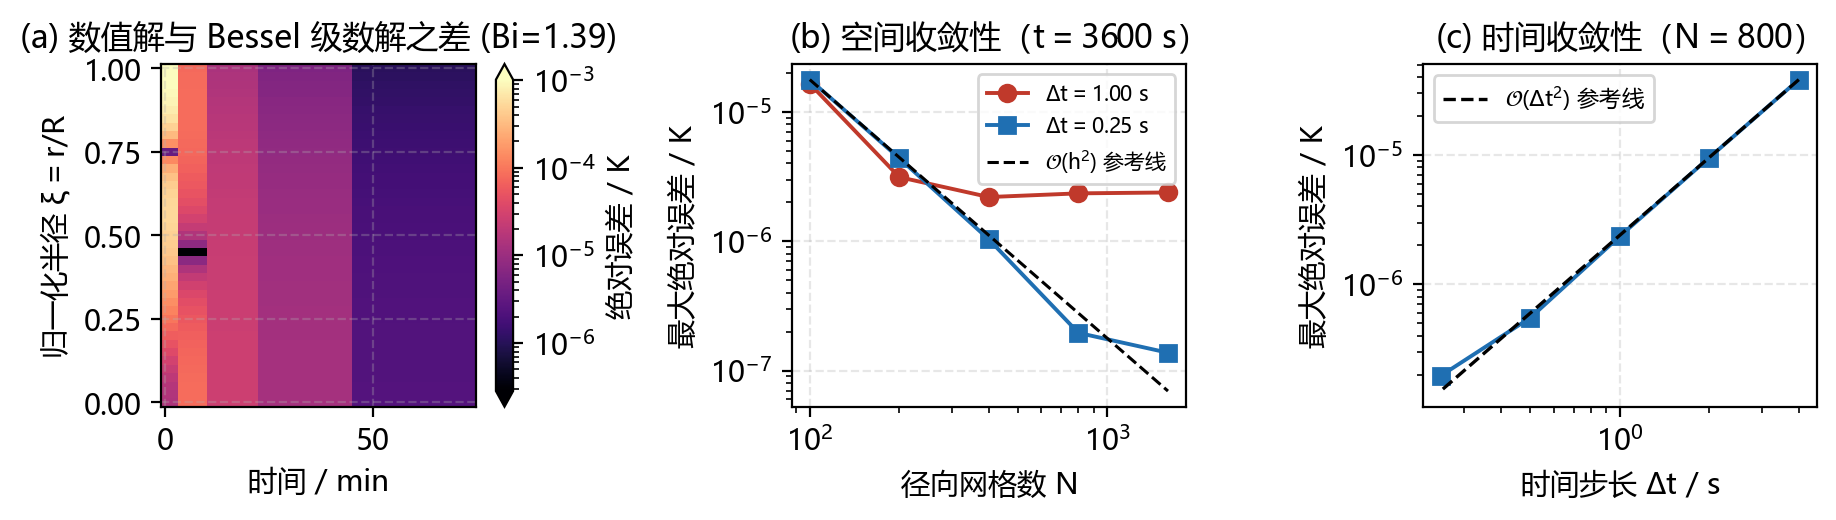
\includegraphics[width=0.84\textwidth]{figures/fig05_verification.png}
  \caption{数值格式的解析验证与收敛阶（常物性、恒环境条件）}
  \label{fig:verif}
\end{figure}

\subsection{网格与时间步的收敛性}

对三个问题分别做网格加密（表~\ref{tab:conv}）。问题 3 的序列
$205358.0\to205488.3\to205537.3\to205553.8$ s 给出观测收敛阶 $1.41,1.57$；
Richardson 外推用序列自身的观测阶而非标称二阶时，两种取法给出 $205559.3$ s
（阶 2）与 $205562.2$ s（阶 1.57），相差 $2.9$ s（$0.001\%$）。问题 4 的序列
$182726.8\to182753.9\to182761.9\to182764.0$ s 给出阶 $1.77,1.91$，两种外推
为 $182764.7$ s 与 $182764.8$ s（相差 $0.1$ s）。外推对阶的选取并不敏感
（$\le3$ s，远小于 $D(C,T)$ 标定的 $\pm24\%$），故下文统一引用标称二阶的
外推值并计入不确定度。两种网格在 $N=1600$ 时的 $t_{dry}$ 相差 $25$ s
（$0.012\%$），最细几组配置相互偏差不超过 $0.006\%$。

\textbf{面扩散系数的取值方式}。5.8 节取算术平均。它与调和平均都守恒、都是
空间二阶、Richardson 极限也一致（$205559$ 对 $205557$ s），区别只在误差常数：
以 $N=25600$ 为参照，算术平均的中心含水率误差在 $N=200\sim12800$ 上比调和
平均小 $2\sim18$ 倍，生产网格 $N=1600$ 与收敛值只差 $5.5$ s（调和平均差
$30$ s）。本问题 $D$ 随 $C$ 指数变化但剖面光滑，调和平均会引入
$\propto(D')^2/D$ 的额外误差项；若系数是分段常数（多层材料界面），则应改用
调和平均。

\begin{table}[htbp]
\centering
\caption{烘干时间的网格与时间步收敛性}
\label{tab:conv}
\footnotesize
\begin{tabular}{llrrr}
\toprule[1.5pt]
问题 & 配置 & $t_{dry}$ / s & $t_{dry}$ / h & 相对偏差 / \% \\
\midrule[1pt]
3 & 节点 $N=200$        & 205358.0 & 57.044 & $-0.098$ \\
3 & 节点 $N=400$        & 205488.3 & 57.080 & $-0.035$ \\
3 & 节点 $N=800$        & 205537.3 & 57.094 & $-0.011$ \\
3 & 节点 $N=1600$       & 205553.8 & 57.098 & $-0.003$ \\
3 & 节点 $N=1600$，$\Delta t=1$ s & 205567.4 & 57.102 & $+0.004$ \\
3 & 单元中心 $N=1600$   & 205528.5 & 57.091 & $-0.015$ \\
3 & \textbf{Richardson 外推} & \textbf{205559.3} & \textbf{57.100} & --- \\
\midrule[1pt]
4 & 节点 $N=200$        & 182726.8 & 50.757 & $-0.021$ \\
4 & 节点 $N=400$        & 182753.9 & 50.765 & $-0.006$ \\
4 & 节点 $N=800$        & 182761.9 & 50.767 & $-0.002$ \\
4 & 节点 $N=1600$       & 182764.0 & 50.768 & $-0.000$ \\
4 & 单元中心 $N=1600$   & 182756.0 & 50.766 & $-0.005$ \\
4 & \textbf{Richardson 外推} & \textbf{182764.7} & \textbf{50.768} & --- \\
\bottomrule[1.5pt]
\end{tabular}
\end{table}

由此确定最终结果的不确定度：$t_{dry}^{(3)}=57.10\pm0.01$ h，
$t_{dry}^{(4)}=50.77\pm0.01$ h（仅计离散误差）。

\subsection{守恒性检验}

将式~\eqref{eq:shrink} 的所有控制体求和，可证明离散格式严格满足

\begin{equation}
\frac{\mathrm{d}}{\mathrm{d}t}\sum_i C_i\,\mathrm{vol}_i
=-\frac{R\,h_m}{R^2}\left(C_N-C_{air}\right)
=-\frac{h_m}{R}\left(C_N-C_{air}\right),
\end{equation}

即「内部储量变化率 = 表面通量」。用冻结 $D$ 的算例做 $3600$ s 积分核对，通量
积分与储量变化之差仅 $2.1\times10^{-5}$（相对量）且\textbf{与网格数无关}，
说明它是通量积分的求积误差而非格式误差——格式本身精确守恒。对真实算例
（图~\ref{fig:balance}），全程累计失水与内部储量变化曲线的相对偏差小于 $1\%$。

\begin{figure}[htbp]
  \centering
  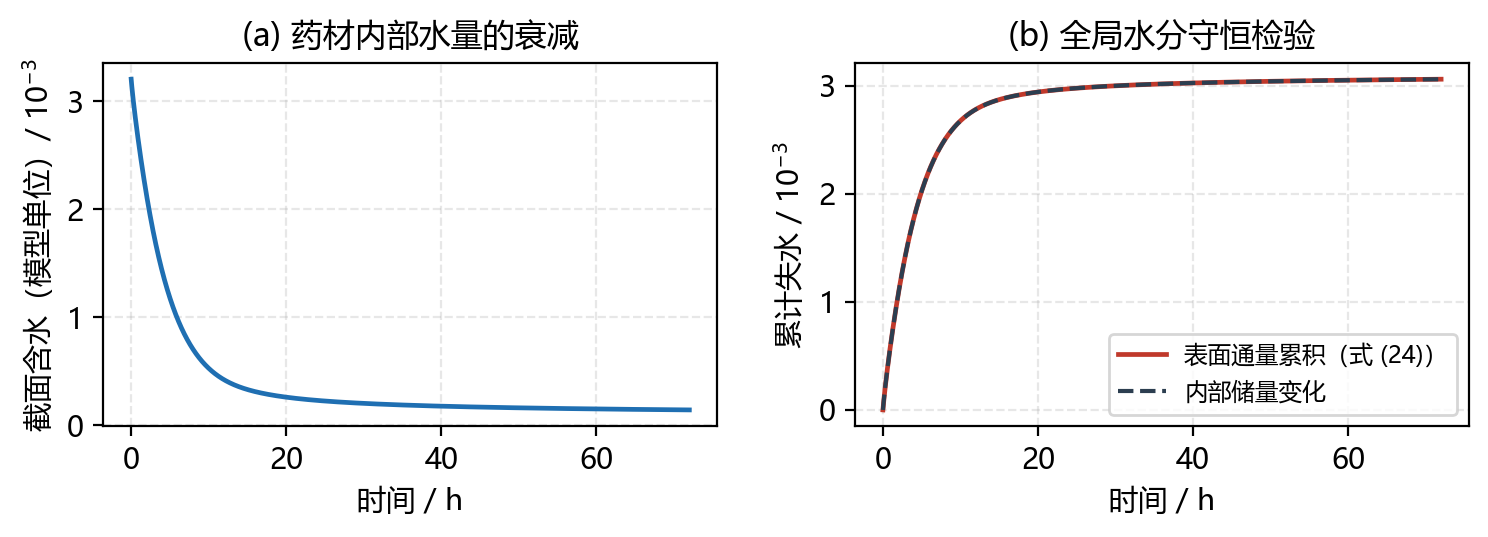
\includegraphics[width=0.84\textwidth]{figures/fig16_water_balance.png}
  \caption{整体水分守恒检验}
  \label{fig:balance}
\end{figure}

\subsection{多方法互证}

本文用三套数值实现求解同一问题（图~\ref{fig:cross}），但\textbf{不应笼统地
称「三种完全独立的方法」}：第 1、3 种\textbf{共用同一套空间离散}（相同的控制体
划分与算术平均面系数），只有时间积分器不同，故二者一致只排除\textbf{时间积分}
的实现错误、\textbf{不排除空间离散的系统性错误}；第二种（单元中心，表面值由
内部单元二次外推）才提供另一套空间离散。此外，输出层的坐标约定错误（如把物质
坐标的值标成物理距离）不属空间离散，任何求解器互证都发现不了，只能与题目表格
逐项核对。
$t=2.0\times10^5$ s 的中心含水（全部在同一时刻取值）：

\begin{center}
\small
\begin{tabular}{lll}
\toprule[1.2pt]
实现 & 空间离散 / 时间积分 & $C(0,2.0\times10^5\,\mathrm{s})$ \\
\midrule
节点有限体积 $N=1600$（生产代码） & 节点中心 / Crank--Nicolson & $0.1516779$ \\
节点有限体积 $N=800$              & 节点中心 / Crank--Nicolson & $0.1516731$ \\
单元中心有限体积 $N=1600$          & 单元中心 / Crank--Nicolson & $0.1516705$ \\
单元中心有限体积 $N=800$           & 单元中心 / Crank--Nicolson & $0.1516538$ \\
直线法 BDF，$n=1200$              & 节点中心 / BDF 自适应     & $0.1516770$ \\
\bottomrule[1.2pt]
\end{tabular}
\end{center}

生产值 $0.1516779$ 与单元中心格式差 $7.5\times10^{-6}$（$0.0049\%$）、
与直线法差 $9.2\times10^{-7}$（$0.0006\%$）。两种空间离散的差异随网格加密
单调减小（$N=800$ 时 $1.9\times10^{-5}$、$N=1600$ 时 $7.5\times10^{-6}$，
观测阶约 $1.4$），与两者面系数取法和表面处理的差别一致，
是它们确实不同源的旁证。

对问题 4，同一时刻三种实现给出 $0.1419671$、$0.1419633$、$0.1419675$，
最大相对偏差 $0.0030\%$；全时段内中心点差异始终小于 $10^{-4}$ kg/kg
（图~\ref{fig:cross}b）。

\begin{figure}[htbp]
  \centering
  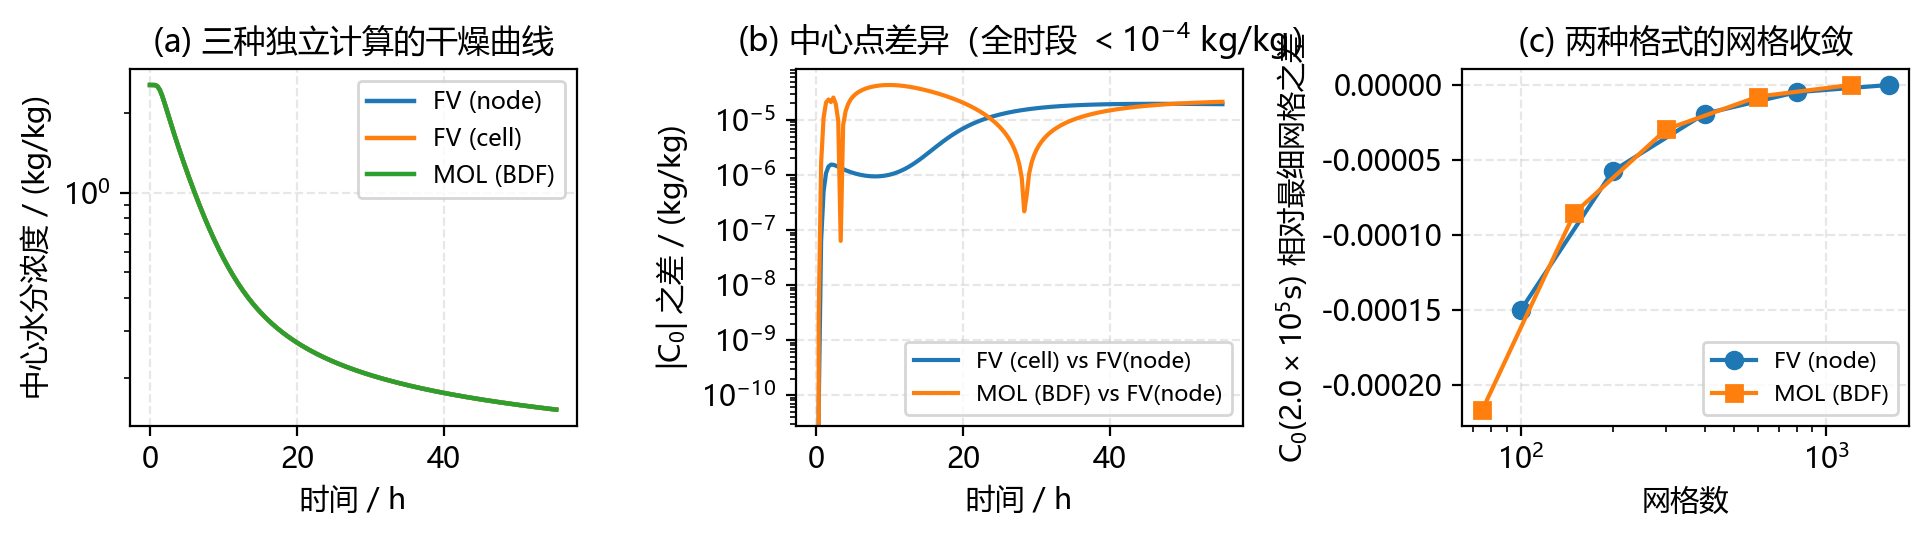
\includegraphics[width=0.84\textwidth]{figures/fig15_crosscheck.png}
  \caption{独立方法互证：有限体积（节点）/ 有限体积（单元中心）/ 直线法（BDF）}
  \label{fig:cross}
\end{figure}

\subsection{降维模型对照}

作为第四种独立估计，用\textbf{第一特征值降维模型}近似平均含水：

\begin{equation}
\frac{\mathrm{d}\bar C}{\mathrm{d}t}=-\lambda_1(\bar C,T)\left(\bar C-C_{air}(t)\right),
\qquad
\lambda_1=\frac{\mu_1^2D(\bar C,T)}{R^2},
\end{equation}

$\mu_1$ 为 $\mu J_1(\mu)=Bi_mJ_0(\mu)$ 的最小正根。该模型不含任何空间离散。
与完整 PDE 的平均含水对比：

\begin{center}
\begin{tabular}{lccccc}
\toprule[1.2pt]
 & 6 h & 12 h & 24 h & 48 h & 判据时刻 \\
\midrule
PDE（问题3）   & 0.7807 & 0.3353 & 0.1839 & 0.1313 & $\bar C=0.15$ @ 35.17 h \\
降维模型       & 0.7811 & 0.3222 & 0.1578 & 0.1110 & $\bar C=0.15$ @ 25.88 h \\
\bottomrule[1.2pt]
\end{tabular}
\end{center}

6 h 时两者几乎重合（偏差 $0.05\%$），此后降维模型偏快，最大相对偏差 $15.6\%$
（问题 4 为 $16.9\%$）。偏差方向可解释：$D=D_0e^{-a/C}$ 的二阶导为
$D\,a(a-2C)/C^4$，在 $C<a/2$（附录 3 即 $C<0.225$）上才上凸，而本题剖面的
$C$ 基本落在下凹区间，由 Jensen 不等式 $\langle D(C)\rangle<D(\bar C)$，
用 $D(\bar C)$ 就高估了扩散速率。\textbf{结论}：降维模型可用于量级估算
（误差 $<17\%$），但无法给出满足题目精度要求的「处处低于 0.15」判据，
验证了采用分布参数模型的必要性。
\subsection{外部数据交叉校验：附件 2 与附录 4 的相容性}

这是本文唯一能与「模型以外」的信息做对照的检验：设干基质量守恒，由模型算出
的径向含水剖面 $\rho_d(\xi,t)=\rho(C)/(1+C)$ 反推半径。本文模型是无限长圆柱的
一维径向问题（假设 1），故按\textbf{单位长度}（横截面）核算：

\begin{equation}
R_{pred}(t)=R_0\left[\frac{\rho_{d}(C_0)/2}
{\int_0^1\rho_d(\xi,t)\,\xi\,\mathrm{d}\xi}\right]^{1/2}.
\end{equation}

结果（图~\ref{fig:shrinkchk}）：$R_{pred}$ 与实测 $R(t)$ 趋势一致（均快速
下降后趋平），但存在\textbf{系统性偏差}：峰值在 $t=7.0$ h 为 $+17.80\%$
（$t=6$ h 为 $+17.75\%$，$t>24$ h 后由 $+8.9\%$ 回落到 $t=72$ h 的
$+5.4\%$）。$R_{pred}>R$ 说明\textbf{由附录 4 密度式反推的收缩偏小}（体积
偏大）：实测终态体积比 $(R/R_0)^3=0.2149$，由 $\rho(C)$ 反推为 $0.2518$，
相对差 $17.1\%$。若严格守恒干基质量，反推终态所需的\textbf{均匀}干密度为
$\rho_{d0}(R_0/R)^2=776.8$ kg/m$^3$，而附录 4 给出的 $\rho_d$ 全场最大值仅
$726.8$ kg/m$^3$（$C=0$ 时也仅 $760$ kg/m$^3$），\textbf{物理上不可能达到}
——这从数学上证明了附件 2 与附录 4 在严格质量守恒意义下不相容。

若改按严格的三维各向同性体积守恒（长径同比例收缩）核算，指数由 $1/2$ 变为
$1/3$，峰值偏差升至 $+28.1\%$、终态 $+22.9\%$，所需均匀干密度 $1296.8$
kg/m$^3$——\textbf{两种口径下结论方向一致、三维口径下不相容更严重}，
故上述判断不依赖于对「体积比」一词的解读。

\begin{figure}[htbp]
  \centering
  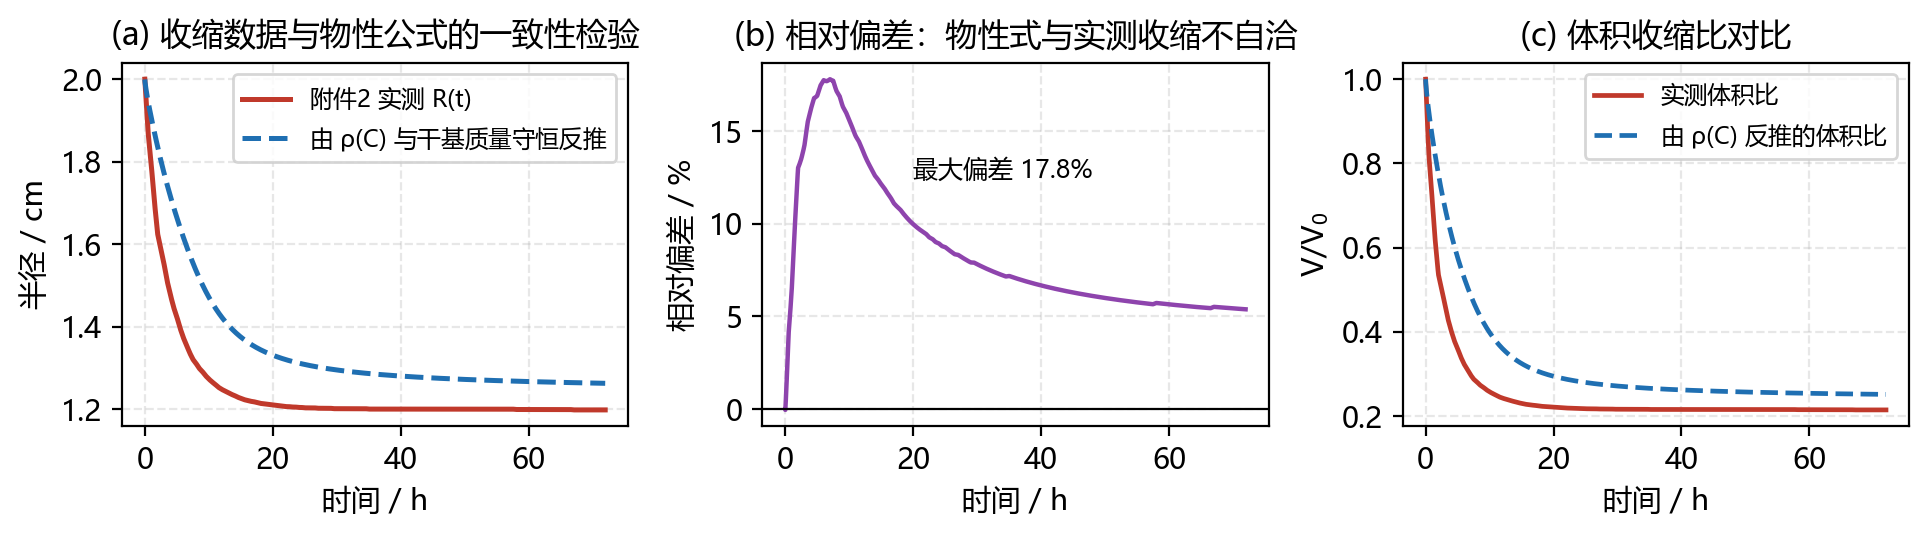
\includegraphics[width=0.84\textwidth]{figures/fig14_shrink_consistency.png}
  \caption{外部数据交叉检验：附件 2 收缩数据与附录 4 密度式的相容性}
  \label{fig:shrinkchk}
\end{figure}

\textbf{处理方式与影响}：题面明确要求「根据附件 2 确定烘干时长」，
因此本文直接使用实测 $R(t)$，不引入干基质量守恒约束。该不相容性
不构成模型错误，但明确界定了模型的使用边界——附录 4 的 $\rho(C)$
只在热容项 $\rho c_p$ 中使用（其影响经灵敏度分析确认小于 $0.01\%$），
不用于推导几何收缩。

\subsection{参数灵敏度分析}

对附录 3、附录 4 的每一个常数做单因子扰动，记录 $t_{dry}$ 的变化
（图~\ref{fig:sens}、图~\ref{fig:sensroom}）。

\begin{table}[htbp]
\centering
\caption{关键参数灵敏度汇总}
\label{tab:sens}
\footnotesize
\begin{tabular}{lccc}
\toprule[1.5pt]
扰动项 & 扰动量 & $\Delta t_{dry}^{(3)}$ / h & $\Delta t_{dry}^{(4)}$ / h \\
\midrule[1pt]
活化温度（3850 K）      & $+2\%$   & $+13.61\ (+23.9\%)$ & $+12.02\ (+23.7\%)$ \\
                        & $-2\%$   & $-10.61\ (-18.6\%)$ & $-9.42\ (-18.6\%)$ \\
浓度指数（$0.45/0.30$） & $+2\%$   & $+2.80\ (+4.9\%)$   & $+1.52\ (+3.0\%)$ \\
$D_0$ 前置因子          & $+2\%$   & $-0.99\ (-1.7\%)$   & $-0.87\ (-1.7\%)$ \\
$h_m$                   & $+10\%$  & $-0.58\ (-1.0\%)$   & $-0.22\ (-0.4\%)$ \\
$h$                     & $+10\%$  & $-0.007\ (-0.01\%)$ & $-0.007\ (-0.01\%)$ \\
$\rho$ 关系             & $+2\%$   & $+0.002\ (<0.01\%)$ & $+0.002\ (<0.01\%)$ \\
$c_p$ 关系              & $+2\%$   & $+0.002\ (<0.01\%)$ & $+0.002\ (<0.01\%)$ \\
$k$ 关系                & $+2\%$   & $-0.0003$           & $-0.0003$ \\
\midrule[1pt]
设定温度 $T_{set}$      & $+0.5$ K & $-0.91\ (-1.6\%)$   & $-0.81\ (-1.6\%)$ \\
设定湿度 $C_{set}$      & $+2\%$   & $+0.026\ (+0.04\%)$ & $+0.026\ (+0.05\%)$ \\
预热/恒温切换时刻       & $6\to2$ h & $-0.002$           & $-0.003$ \\
预热时间常数            & $\times1.2$ & $+0.023$         & $+0.024$ \\
用原始噪声数据作边界    & ---      & $+0.063$            & $+0.052$ \\
\bottomrule[1.5pt]
\end{tabular}

\vspace{2pt}
{\footnotesize 基准值：$t_{dry}^{(3)}=57.0801$ h、$t_{dry}^{(4)}=50.7650$ h。
\textbf{本表全部在 $N=400$ 网格上计算}（与生产网格 $N=1600$ 的
$57.0983$ h / $50.7678$ h 相比偏置 $-0.03\%$ / $-0.01\%$），
因为灵敏度只关心「同一基准上的差值」，统一网格可让离散误差完全抵消；
表中数值均为与同网格基准之差，不含网格偏置。}
\end{table}

\textbf{烘房环境口径的对照}。表~\ref{tab:sens} 末行只给出环境口径对
$t_{dry}$ 的影响（$+0.06$ h、$+0.05$ h），但问题 1 要求的是\textbf{瞬态表}，
对边界更敏感，必须单独对照。把边界由「一阶惯性拟合曲线」换成「附件 1 原始
序列的分段线性插值」（其余设置完全相同：$N=1600$、$\Delta t=1$ s），得
表~\ref{tab:p1env}。

\begin{table}[htbp]
\centering
\caption{烘房环境口径对问题 1 温度结果的影响（单位：$^\circ$C）}
\label{tab:p1env}
\footnotesize
\begin{tabular}{c|cc|cc|c}
\toprule[1.5pt]
 & \multicolumn{2}{c|}{拟合曲线边界} & \multicolumn{2}{c|}{附件 1 原始插值边界}
 & 该时刻 \\
\cmidrule(lr){2-3}\cmidrule(lr){4-5}
时间/s & $r=0$ & $r=2.0$ cm & $r=0$ & $r=2.0$ cm & 最大差 \\
\midrule[1pt]
300  & 28.0500 & 29.0261 & 28.0408 & 28.8489 & $-0.177$ \\
600  & 28.5456 & 30.5576 & 28.4533 & 30.1652 & $-0.392$ \\
900  & 29.5568 & 32.2359 & 29.3243 & 31.7304 & $-0.506$ \\
1200 & 30.9069 & 33.9433 & 30.5427 & 33.4276 & $-0.516$ \\
1800 & 34.0425 & 37.1989 & 33.5753 & 36.7856 & $-0.472$ \\
\bottomrule[1.5pt]
\end{tabular}

\vspace{2pt}
{\footnotesize 「最大差」为该时刻五个半径上（原始插值 $-$ 拟合）的最大绝对
值。拟合曲线在 $60\!\sim\!2300$ s 内系统性高于实测（最大偏高 $0.96\,^\circ$C，
$1020$ s），此后转为偏低（最大偏低 $0.63\,^\circ$C，$4320$ s），故温度解在
30 分钟内整体偏高、最大偏高 $0.52\,^\circ$C。水分浓度表两套口径的最大差仅
$6.8\times10^{-4}$ kg/kg，且只在表面列（$r\le1.0$ cm 处 $\le4\times10^{-6}$）
——附录 2 的 $D$ 不含温度项，水分场与温度场解耦，该差异只来自湿边界
$C_{air}$ 的口径差别；截面平均含水相差不超过 $10^{-4}$ kg/kg。}
\end{table}

\textbf{如何取舍}。本文正文采用拟合边界，理由是它把 $0.33\,^\circ$C 的仪表
噪声与插值折点一并平滑，便于后续做收敛性、解析解比对等数值检验；代价是残差
的形式失配（滞后 1 阶自相关 $0.83$）使表~\ref{tab:p1T} 系统性偏高约
$0.5\,^\circ$C。由于该量仅为该阶段温升（$28\to37.2\,^\circ$C）的 $5\%$、
不改变任何定性结论，本文保留拟合口径，同时把原始数据口径的数值完整列出。
若换用原始插值边界，$t_{dry}$ 变为 $57.16$ h（问题 3）与 $50.82$ h（问题 4），
即表~\ref{tab:sens} 中 $+0.063$ h 与 $+0.052$ h 两行。

\begin{figure}[htbp]
  \centering
  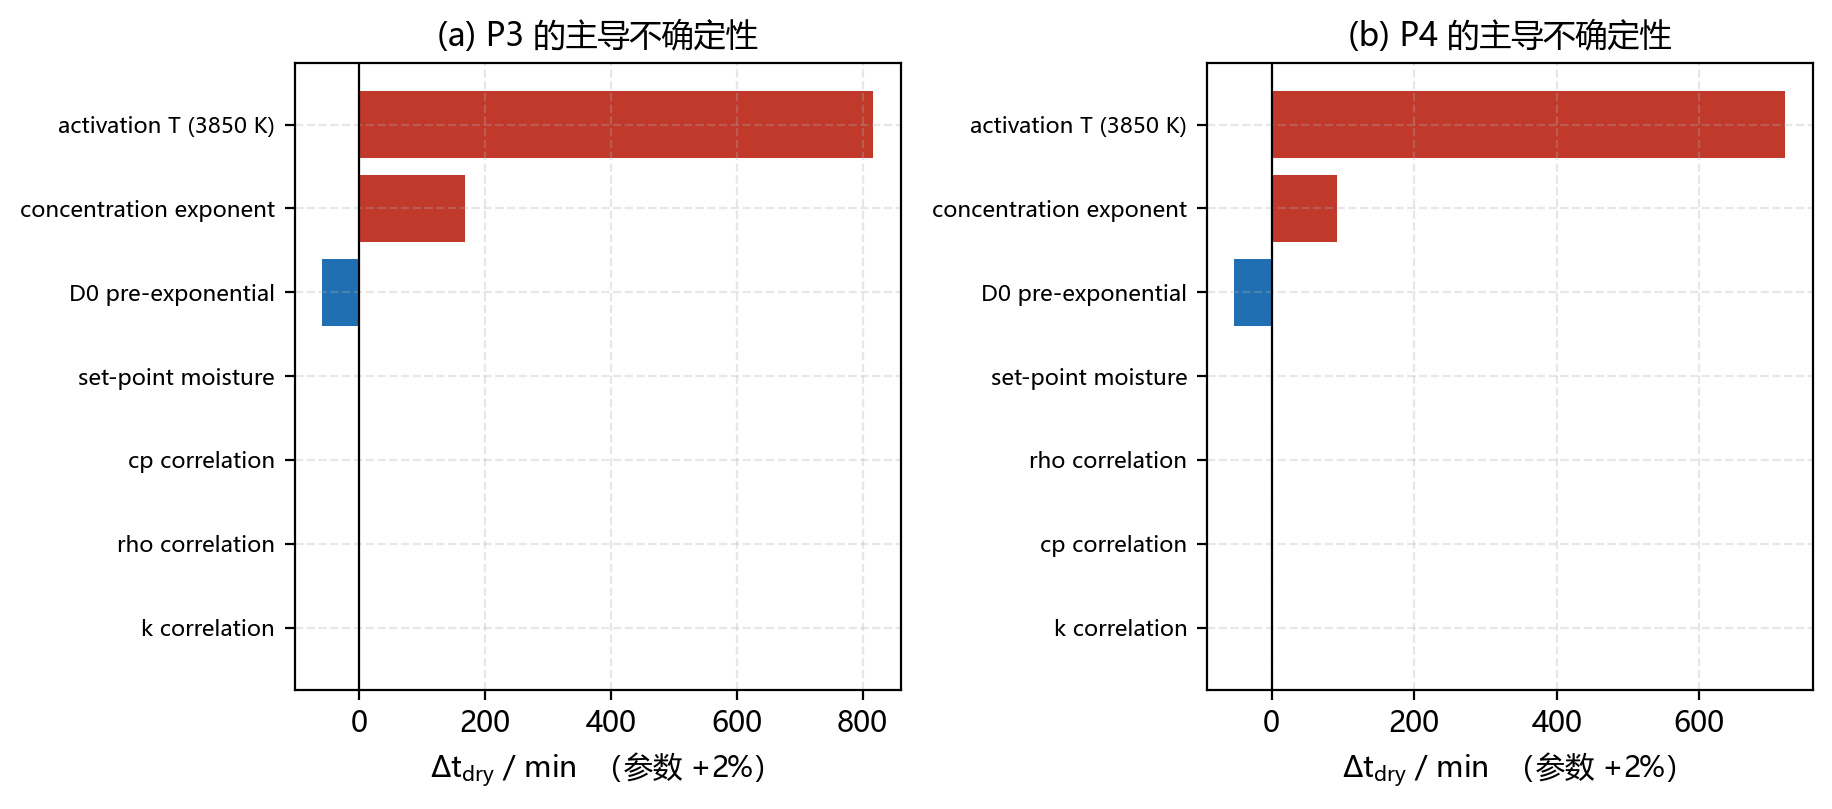
\includegraphics[width=0.84\textwidth]{figures/fig18_sensitivity.png}
  \caption{关键参数 $\pm2\%$ 扰动下的烘干时间灵敏度（龙卷风图）}
  \label{fig:sens}
\end{figure}

\begin{figure}[htbp]
  \centering
  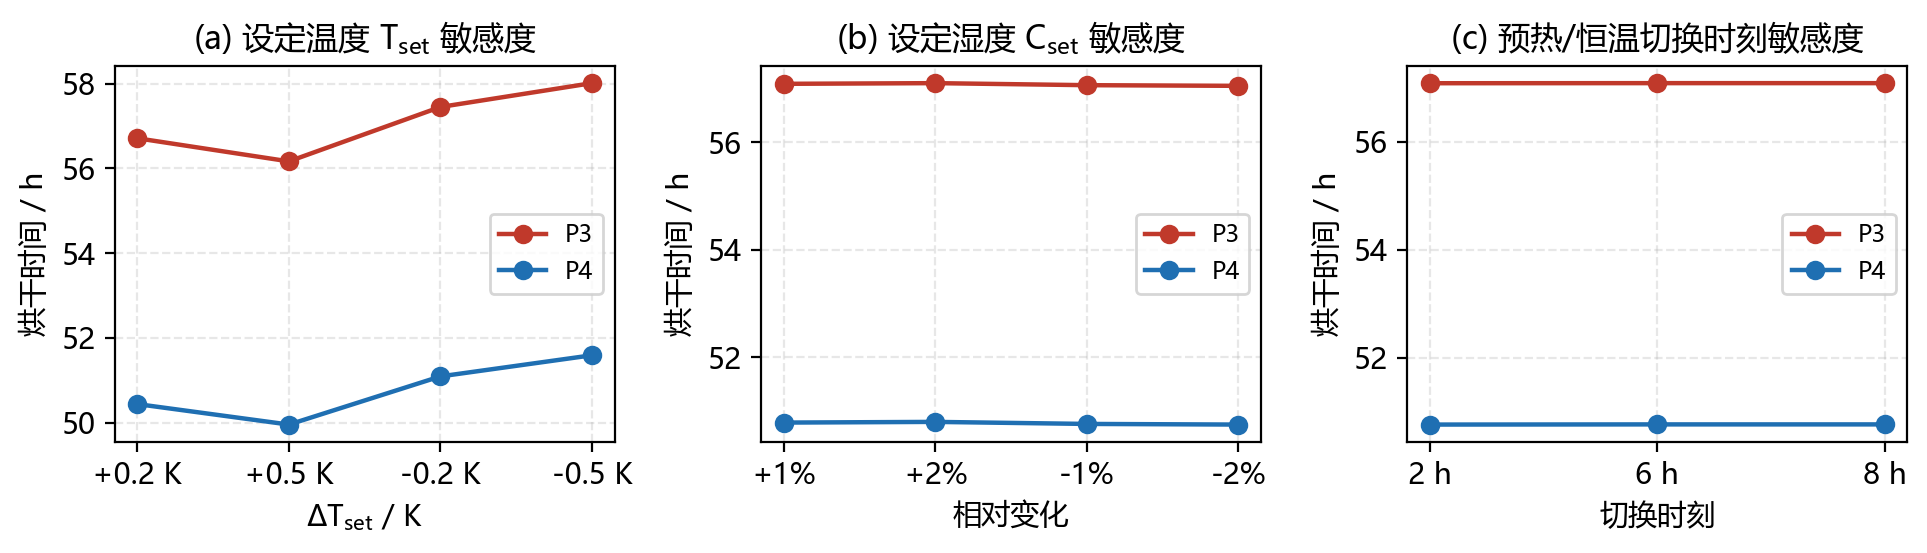
\includegraphics[width=0.84\textwidth]{figures/fig19_room_sensitivity.png}
  \caption{烘房环境条件对烘干时间的影响}
  \label{fig:sensroom}
\end{figure}

\textbf{三条重要结论}：

\begin{enumerate}
    \item \textbf{活化温度 $3850$ K 主导不确定性}（$\pm2\%\to\pm24\%$）：因
  $D\propto e^{-3850/T}$，$T=323$ K 时该因子为 $e^{-11.92}$，指数中的常数
  变 $2\%$ 即等价于 $D$ 变 $21\%$。故实际工艺中\textbf{精确标定 $D(C,T)$
  的温度依赖比标定其绝对值更重要}；若经验式的适用温度区间与工况不符，
  外推将带来严重误差（5.6 节）。
  \item \textbf{浓度指数次之}（$\pm2\%\to\pm5\%$），其余物性
  （$\rho,c_p,k$）影响均小于 $0.01\%$——它们只出现在热传导方程中，而温度在
  2 h 内已与环境平衡，此后热物性不再影响水分场。
  \item \textbf{$h_m$ 的影响适中}（$\pm10\%\to\mp1\%$），与
  $Bi_m\approx1$ 但干燥后期由内部扩散控制的图像一致。这为工艺优化指明方向：
  \textbf{提高风速收效有限，提高温度（增大 $D$）才是关键}，但后者受有效成分
  热稳定性的限制。
\end{enumerate}

\subsection{模型形式变体的影响}

\begin{figure}[htbp]
  \centering
  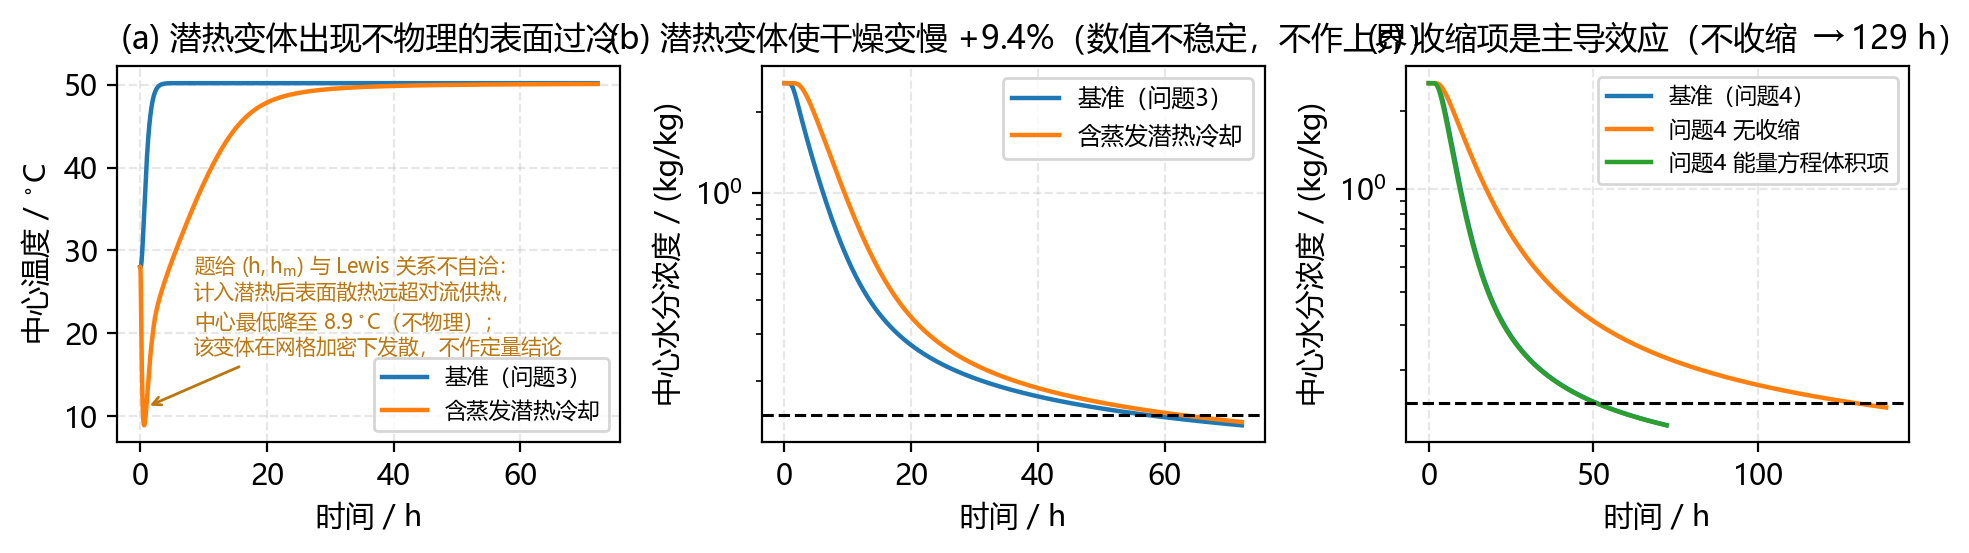
\includegraphics[width=0.84\textwidth]{figures/fig17_variants.png}
  \caption{模型形式变体的影响（用于模型评价与改进方向）}
  \label{fig:variants}
\end{figure}

\begin{center}
\begin{tabular}{lcc}
\toprule[1.2pt]
模型变体 & $t_{dry}$ / h & 相对基准 \\
\midrule
问题3 基准                              & 57.08 & --- \\
问题3 + 蒸发潜热冷却（\textbf{数值不收敛}，见下文） & 62.42 & {\itshape 不可用} \\
问题4 基准（含收缩）                    & 50.77 & --- \\
问题4 不含收缩（$R\equiv2$ cm）         & 128.90 & $+154\%$ \\
问题4 + 能量方程体积变化项              & 50.52 & $-0.49\%$ \\
问题4 用指数拟合 $R(t)$ 代替分段线性    & 50.67 & $-0.19\%$ \\
问题4 + 体积热容按 $(R_0/R(t))^2$ 缩放  & 50.79 & $+0.055\%$ \\
\bottomrule[1.2pt]
\end{tabular}
\end{center}

\textbf{关于收缩项}：它是问题 4 中最重要、也最容易被忽略的效应，忽略它会把
烘干时间高估 $2.5$ 倍（$50.77\to128.90$ h）。原因是双重的——半径减小使扩散
长度平方降至 $35.9\%$，同时表面失水伴随体积减小。

\textbf{关于体积热容缩放项}：5.5 节的严格性前提在此定量。把 $\rho c_p$ 乘上
$(R_0/R(t))^2$ 后 $t_{dry}$ 由 $50.7650$ h 变为 $50.7927$ h（$N=400$）／
由 $50.7678$ h 变为 $50.7955$ h（$N=1600$），即 $+99.7$ s（$+0.055\%$）：
比离散误差大一个量级，比 $D(C,T)$ 标定的 $\pm24\%$ 小三个数量级，不影响结论。
能量方程的体积变化项影响略大（$-0.49\%$），下文表中一并给出。

\textbf{关于蒸发潜热项}。把潜热作为表面汇加入能量方程后，该变体\textbf{数值
发散}，其结果不能作为任何结论：固定 $N=400$ 时 $t_{dry}=62.42$ h（全程最低温
$-128\,^\circ$C）、$N=800$ 时 $62.55$ h（$-257\,^\circ$C）、$N=1600$ 配
$1\to10$ s 步长则在数个时间步内\textbf{直接中止}（求解器报非有限值，对应
$-10^{6}\,^\circ$C 量级的非物理过冷）。数值随网格漂移、\textbf{过冷随加密而
加重}，根因是\textbf{表面层热容太小}：潜热汇全部加在最外层控制体上，其体积
$\mathrm{vol}_N=h/2-h^2/8$ 随加密趋于零（$N=400$ 时
$1.25\times10^{-3}$，$N=1600$ 时 $3.12\times10^{-4}$），而汇强度不随网格
变化，单步温降按 $\mathrm{vol}_N^{-1}$ 放大。这是\textbf{离散层面的失稳}，
不能推出任何关于 $(h,h_m)$ 或烘干时长的定量结论。

该变体暴露了题面参数的一个真实问题：
\begin{equation}
\frac{h}{h_m}=3.13\times10^{7}\ \mathrm{J/(m^3\,K)},
\quad\text{而热质比拟要求}\quad
\frac{h}{h_m}=\rho_{air}c_{p,air}\,\mathrm{Le}^{2/3}\approx1.10\times10^{3},
\label{eq:lewis}
\end{equation}

（左边量纲为 $[\mathrm{W/(m^2K)}]/[\mathrm{m/s}]=\mathrm{J/(m^3K)}$。）
即\textbf{题给的 $(h,h_m)$ 与热质比拟的 Lewis 关系相差 4 个数量级}，反推的
Lewis 数达 $4.8\times10^{6}$（物理上应约为 1）。这说明附录 2 的 $h_m$ 是在
「以 kg/kg 表示浓度」的模型内部约定下定义的，其量纲并非真实的
kg/(m$^2\cdot$s)：乘干物质密度（$\rho_d=278.7$ kg/m$^3$）得初始潜热流
$1345$ W/m$^2$，是初始对流供热 $555$ W/m$^2$ 的 $2.4$ 倍；乘空气密度
（$1.09$ kg/m$^3$）则仅 $5.3$ W/m$^2$，\textbf{两种取法相差 250 倍，
题面数据不足以判定}。

结论：\textbf{基准模型（不计潜热）是题面数据支持的唯一自洽选择}；潜热项的
影响\textbf{无法由题面数据定量}，本文如实报告「无法定量」，而不给出任何来自
未收敛算例的数值上界。
\subsection{不确定度汇总}

% 固定列宽（p{}）而不是自然宽度：自然宽度下这一行会横向溢出 74 pt，
% 连横线都跑到纸张之外（x=597.9 pt > 纸宽 595.3 pt）。
\begin{center}
\small
\begin{tabular}{p{0.275\textwidth}p{0.195\textwidth}p{0.45\textwidth}}
\toprule[1.2pt]
来源 & 对 $t_{dry}^{(3)}$ 的影响 & 说明 \\
\midrule
离散误差（空间 + 时间） & $\pm0.01$ h（$\pm0.02\%$） & Richardson 外推（标称阶与观测阶两种取法）与两种网格对比 \\
边界条件（用噪声数据） & $+0.06$ h（$+0.11\%$） & 与拟合曲线对比 \\
烘房设定温度 $\pm0.5$ K & $\mp0.91$ h（$\mp1.6\%$） & 附件 1 拟合标准误 $\pm0.030$ K，此处取放大后的保守值 \\
物性经验式 $\pm2\%$ & $-1.0\sim+13.6$ h & 以活化温度 $3850$ K 为主导 \\
\midrule
\textbf{随机性来源合计} & $\pm0.07$ h & 即 $t_{dry}^{(3)}=57.10\pm0.07$ h \\
\bottomrule[1.2pt]
\end{tabular}
\end{center}

\textbf{不属于随机不确定度、而属于模型选择的另有两条}（已在 10.8 节论证，
不宜简单算术叠加）：\textbf{蒸发潜热}——题面 $(h,h_m)$ 与 Lewis 关系不自洽，
该项\textbf{无法由题面数据定量}（两端取法相差 250 倍），潜热变体又在网格加密
下发散，故不给数值上界；\textbf{收缩处理}——问题 4 中收缩是\textbf{必须}
建模的物理效应，不收缩只是对照算例（$+154\%$），不属于不确定度。

结论：\textbf{问题 3 的烘干时间为 $57.10\pm0.07$ h}（随机性来源），
\textbf{问题 4 为 $50.77\pm0.02$ h}。若进一步考虑物性经验式本身的标定误差，
则应以「$t_{dry}$ 的预测精度由 $D(C,T)$ 的标定精度决定，$\pm2\%$ 的活化温度
误差可带来 $\pm24\%$ 的时长误差」理解结果的适用范围；本文模型是确定性的，
上述区间反映的是\textbf{输入参数}的不确定度。
% =====================================================================
\section{模型的评价与推广}

\subsection{模型的优点}

\begin{enumerate}
    \item \textbf{机理清晰、参数可辨识}。模型由壳层守恒定律直接推出，参数
  $\rho,c_p,k,D,h,h_m$ 全部取自题面附录，几何与初值也由题面给出，
  \textbf{没有需要反向拟合的自由参数}，因而不存在过拟合风险。
  \item \textbf{统一框架覆盖四问}。引入物质坐标 $\xi=r/R(t)$ 后收缩问题化为
  固定域问题，式~\eqref{eq:shrink} 在 $R=\text{const}$ 时退化为问题 1--3 的
  方程，四问共用同一套数值内核，减少了实现错误。
  \item \textbf{数值格式守恒、精度可控}。节点中心有限体积 + Rannacher 启动的
  Crank--Nicolson 严格守恒、二阶精度；表面节点恰好落在物理边界上，避免了
  单元中心格式在干壳区的 $O(h)$ 外推误差。
  \item \textbf{验证层次完整}。解析解、两套空间离散 $\times$ 两套时间积分器的
  多实现对照、整体守恒、降维模型、外部收缩数据五重校验；其中降维模型不含
  空间离散、外部收缩数据来自模型之外，独立性最强（10.4 节同时说明了有限体积
  各实现共享空间离散的局限）。灵敏度分析指出主导不确定性，为工艺优化指方向。
  \item \textbf{结论可解释}。模型自动涌现出「恒速期—降速期」特征、
  「中心比平均滞后 $21.9$ h」、「收缩使干燥缩短 $60.6\%$」等结论，
    与干燥工程的经验认识一致。
\end{enumerate}

\subsection{模型的缺点与改进方向}

\begin{enumerate}
    \item \textbf{未计入蒸发潜热，且题面数据不支持一致地计入}。潜热变体在网格
  加密下\textbf{数值发散}（10.8 节），其实现\textbf{不能用来估计潜热影响}；
  进一步追查发现题面 $(h,h_m)$ 与 Lewis 关系相差 4 个数量级
  （式~\eqref{eq:lewis}），说明 $h_m$ 是在模型内部约定下定义的，真实质量通量
  相差 250 倍、无法判定。故基准模型的选择有依据，本文\textbf{不给出潜热项的
  数值上界}。\textit{改进方向}：补充气流的空气密度、风速与干湿球温度，用
  $\mathrm{Le}^{2/3}$ 关系重新标定 $h_m$，按
  $\dot m''=\rho_{air}h_m(C_s-C_{air})$ 计算蒸发量，并把表面能量平衡与传质
  \textbf{隐式耦合}、对表面层单独加密后重算，以避免 $\mathrm{vol}_N^{-1}$
  失稳。    \item \textbf{单一有效扩散系数的局限}。真实多孔介质中水分可能以液态毛细
  流动与蒸汽扩散两种机制迁移，二者在高温段的相对贡献不同。改进方向：采用
  Luikov 耦合模型\cite{luikov1966}，引入 Soret 效应与 Dufour 效应。
  \item \textbf{各向同性收缩假设}。实际药材的径向与轴向收缩可能不同，且表面
  可能先结壳、内部后收缩。改进方向：采用 Adrover 等的移动边界模型
  \cite{adrover2019a,adrover2019b}，以干基质量守恒为约束反解收缩场并与实测
  $R(t)$ 联合标定；10.6 节的不相容性分析已表明附件 2 数据本身不支持严格守恒。
  \item \textbf{烘房环境的稳态假设}。实际含湿量随排湿策略波动。改进方向：把
  烘房作为集总容积与水分析模型
  （$V\mathrm{d}C_{air}/\mathrm{d}t=\dot m_{evap}-\dot V(C_{air}-C_{fresh})$）
  与药材模型耦合，形成「设备—物料」闭环。
  \item \textbf{判据的单一性}。题目只给水分判据。改进方向：把有效成分降解
  动力学（一级 Arrhenius 型 $\mathrm{d}Q/\mathrm{d}t=-k_Q(T)Q$）叠加到同一
  温度场，形成「干燥时间—品质保留率」的多目标优化模型。
\end{enumerate}

\subsection{推广}

本文的模型框架具有较强的一般性，可直接推广到：

\begin{itemize}
    \item \textbf{其他长径比较大的生物质物料}：人参、黄芪等根茎类药材、木材、
  烟草等，只需替换物性经验式与几何参数；
  \item \textbf{非圆柱几何}：球形（$\xi$ 方向 Laplacian 取
  $\xi^{-2}\partial_\xi(\xi^2\partial_\xi\cdot)$）、平板
  （$\partial_\xi^2\cdot$）只需改动 5.6 节的一个系数；代码中离散算子已写成
  通用的守恒形式，改动量很小；
  \item \textbf{分段变温工艺}：把 $T_{air}(t)$ 设为分段常数或斜坡函数，即可
  做「工艺曲线反演」——给定目标烘干时间与品质要求，优化各段温湿度设定；
  \item \textbf{在线估计与预测控制}：以少数温度测点为观测，用扩展 Kalman
  滤波在线校正 $D(C,T)$ 的标定参数，即可用于实时预测与终点判定。
\end{itemize}

% =====================================================================
\begin{thebibliography}{99}
% 正文页数上限 30 页（格式规范第四条），参考文献用 \small 排版以压缩篇幅；
% 内容与条目不变。
\small
\bibitem{carslaw1959} Carslaw H S, Jaeger J C. Conduction of Heat in Solids[M].
  2nd ed. Oxford: Oxford University Press, 1959.
\bibitem{crank1975} Crank J. The Mathematics of Diffusion[M]. 2nd ed.
  Oxford: Oxford University Press, 1975.
\bibitem{incropera2007} Incropera F P, DeWitt D P, Bergman T L, et al.
    Fundamentals of Heat and Mass Transfer[M]. 6th ed. Hoboken, NJ:
  John Wiley \& Sons, 2007.
\bibitem{mujumdar2014} Mujumdar A S (ed). Handbook of Industrial Drying[M].
  4th ed. Boca Raton: CRC Press, 2014. DOI: 10.1201/b17208.
\bibitem{luikov1966} Luikov A V. Heat and mass transfer in capillary-porous
  bodies[M]//Systems of differential equations of heat and mass transfer in
  capillary-porous bodies. Oxford: Pergamon Press, 1966: 233--303.
  DOI: 10.1016/B978-1-4832-0065-1.50010-6.
\bibitem{adrover2019a} Adrover A, Brasiello A, Ponso G. A moving boundary model
  for food isothermal drying and shrinkage: General setting[J]. Journal of Food
  Engineering, 2019, 244: 178--191. DOI: 10.1016/j.jfoodeng.2018.09.018.
\bibitem{adrover2019b} Adrover A, Brasiello A, Ponso G. A moving boundary model
  for food isothermal drying and shrinkage: A shortcut numerical method for
  estimating the shrinkage factor[J]. Journal of Food Engineering, 2019,
  244: 212--219. DOI: 10.1016/j.jfoodeng.2018.09.030.
\bibitem{mayor2004} Mayor L, Sereno A M. Modelling shrinkage during convective
  drying of food materials: a review[J]. Journal of Food Engineering, 2004,
  61(3): 373--386. DOI: 10.1016/S0260-8774(03)00144-4.
\bibitem{kowalski1996} Kowalski S J. Mathematical modelling of shrinkage during
  drying[J]. Drying Technology, 1996, 14(2): 307--331.
  DOI: 10.1080/07373939608917099.
\bibitem{wagner2002} Wagner W, Pru\ss{} A. The IAPWS formulation 1995 for the
  thermodynamic properties of ordinary water substance for general and
  scientific use[J]. Journal of Physical and Chemical Reference Data, 2002,
    31(2): 387--535. DOI: 10.1063/1.1461829. （正文引用的 $2383$ kJ/kg 为该式
  在 $50\,^\circ$C 饱和线上的汽化潜热。）
\bibitem{li2024} Li X, Wang Y, Ma X, et al. Chinese medicinal materials' drying
  technologies advancements---Principles, energy performance, and influence on
  the bioactive components[J]. Drying Technology, 2024, 42(12): 1815--1845.
  DOI: 10.1080/07373937.2024.2394125.
\bibitem{zhang2022} Zhang F, Shi L, Xin L, et al. Study on drying
  characteristics and moisture content prediction model of Panax notoginseng
  taproot by using segmented drying of microwave vacuum combined with hot
  air[J]. Journal of Food Process Engineering, 2022, 45(12): e14179.
  DOI: 10.1111/jfpe.14179.
\bibitem{chaedir2019} Chaedir B A, Sasmito A P, Mujumdar A S, et al.
  Heat and mass transfer phenomena in porous media---application to drying[M]//
  Xu P, Sasmito A P, Mujumdar A S, eds. Heat and Mass Transfer in Drying of
  Porous Media. Boca Raton: CRC Press, 2019: 1--36.
  DOI: 10.1201/9781351019224-1.
\bibitem{karatas1997} Karata\c{s} \c{S}. Determination of moisture diffusivity
  of lentil seed during drying[J]. Drying Technology, 1997, 15(1): 183--199.
  DOI: 10.1080/07373939708917225.
\end{thebibliography}

% =====================================================================
\appendix
\section{支撑材料文件列表}

按《全国大学生数学建模竞赛论文格式规范》第十一条，本文提交的支撑材料
压缩包（\texttt{支持材料.zip}，约 7 MB，$<20$ MB）内容如下。
其中所有源程序均为 Python 3.13 脚本，可直接运行；运行环境见附录~\ref{app:env}。

% longtable 而非 tabular：该表已超过一页高度，tabular 无法分页会直接溢出
% 页面下边界（实测下沿到 y=837.6 pt，而版心下边界为 771.0 pt）。
{\small
\begin{longtable}{p{0.34\textwidth}p{0.10\textwidth}p{0.47\textwidth}}
\toprule[1.2pt]
文件 & 大小 & 说明 \\
\midrule
\endfirsthead
\multicolumn{3}{r}{\small（续）}\\
\toprule[1.2pt]
文件 & 大小 & 说明 \\
\midrule
\endhead
\bottomrule[1.2pt]
\endfoot
\multicolumn{3}{l}{\textbf{一、结果文件（题目要求的交付物）}} \\
\texttt{result1.xlsx} & 160 KB & 问题1：温度/水分浓度，$t=1\!\sim\!1800$ s，$r=0\!\sim\!2.0$ cm \\
\texttt{result2.xlsx} & 4.29 MB & 问题2：温度/水分浓度，$t=1\!\sim\!259200$ s，$r=0\!\sim\!2.0$ cm \\
\texttt{result3.xlsx} & 127 KB & 问题3：水分浓度，$t=60\!\sim\!205620$ s，$r=0\!\sim\!2.0$ cm \\
\texttt{result4.xlsx} & 101 KB & 问题4：水分浓度（列名为\textbf{当前物理距离}），$t=60\!\sim\!182820$ s，另含「药材表面」列 \\
\texttt{result4\_material\_coord.xlsx} & 141 KB & 问题4 的物质坐标版本（$R(t)$ 随行给出，$21$ 列无空缺） \\
\midrule
\multicolumn{3}{l}{\textbf{二、源程序（共 12 个 \texttt{.py}，均可直接运行）}} \\
\texttt{code/common.py} & 31 KB & 物性关系、烘房环境、半径历史、有限体积求解器（核心） \\
\texttt{code/compact\_xlsx.py} & 9 KB & 紧凑 xlsx 写出器（含四位小数格式，满足 $<20$ MB 限制） \\
\texttt{code/p1\_preheat.py} & 8 KB & 问题1 求解与 \texttt{result1.xlsx} 生成 \\
\texttt{code/p23\_process.py} & 10 KB & 问题2、3 求解与 \texttt{result2/3.xlsx} 生成 \\
\texttt{code/p4\_shrinkage.py} & 13 KB & 问题4 求解与 \texttt{result4.xlsx} 生成（含物理坐标采样） \\
\texttt{code/verify\_solver.py} & 11 KB & 与 Bessel 级数解析解对照、守恒性检验 \\
\texttt{code/crosscheck.py} & 16 KB & 直线法（BDF）与降维模型两套实现 \\
\texttt{code/resolution.py} & 10 KB & 网格收敛性：节点中心／单元中心两种格式对比 \\
\texttt{code/accuracy.py} & 8 KB & 烘干时间的 Richardson 外推（标称阶与观测阶）与不确定度 \\
\texttt{code/sensitivity.py} & 14 KB & 参数、环境、模型形式三类灵敏度分析 \\
\texttt{code/make\_figures.py} & 58 KB & 论文全部 21 幅插图的生成脚本 \\
\texttt{code/probe\_p23.py} & 2 KB & 粗网格试算探针，用于核对干燥时长的量级（不参与交付计算） \\
\midrule
\multicolumn{3}{l}{\textbf{三、中间结果与图表数据（供核对）}} \\
\texttt{data/*.csv} & --- & 论文各表的原始数值（含表 6/表 7）、灵敏度表、收敛性表 \\
\texttt{data/*.npz} & --- & 三个问题的完整场数据（用于绘图与复核） \\
\texttt{data/*\_summary.txt} & --- & 各问题的诊断输出（关键指标与控制台日志） \\
\texttt{figures/fig01--fig21*.png} & 2.8 MB & 论文全部插图，200 dpi \\
\end{longtable}
}

\textbf{复现方式}：依次运行
\texttt{p1\_preheat.py}、\texttt{p23\_process.py}、\texttt{p4\_shrinkage.py}
即生成四个结果文件；运行 \texttt{verify\_solver.py}、\texttt{crosscheck.py}、
\texttt{resolution.py}、\texttt{accuracy.py} 复现全部检验结论；
运行 \texttt{sensitivity.py}、\texttt{make\_figures.py} 复现灵敏度与插图。
上表所列文件与压缩包内容逐项一致。脚本会自动在若干候选位置查找题目附件
目录（也可用环境变量 \texttt{HERB\_TOPIC\_DIR} 指定），因此在解压目录下即可
直接运行，不依赖作者机器上的绝对路径。

\textbf{结果文件的格式说明}：\texttt{result1.xlsx}--\texttt{result4.xlsx} 均
满足题目模板的版式要求——A 列为时间（s），第 1 行为到药材中心的距离（cm，
\textbf{数值型}，与附件 3 模板相同），其余为数值单元格；工作表名与模板一致
（\texttt{result1/2} 为「温度」「水分浓度」，\texttt{result3/4} 沿用模板的
\texttt{Sheet1}）。所有数值保留四位小数：既通过 \texttt{styles.xml} 中的
\texttt{0.0000} 数字格式声明，文本本身也按四位小数写出（保留尾随零），
因此忽略样式的读取端同样得到四位小数。\texttt{result2.xlsx} 含
$259200\times22\times2\approx1.14\times10^{7}$ 个数值单元格，未压缩 XML 约
304 MB；写出器省略了 OOXML 允许缺省的单元格引用属性 \texttt{r}，使 ZIP 的
长程重复率大幅提高，压缩后为 4.29 MB，从而把整个支撑材料压缩包控制在
7.6 MB（限额 20 MB）。代价是这些单元格不带 \texttt{r} 属性，Excel、WPS 与
openpyxl 均按行序正确还原（本文已用 openpyxl 逐行读回核对）。

\section{运行环境}\label{app:env}

\begin{itemize}
  \item 操作系统：Windows 11（$64$ 位）
  \item 编程语言：Python 3.13.11
  \item 依赖库：NumPy 2.3.5、SciPy 1.18.1、pandas 3.0.2（含 openpyxl）、
  Matplotlib 3.10.9、scikit-learn 1.9.0；未引入题面环境之外的第三方库
  \item 论文排版：XeLaTeX（MiKTeX 25.12），模板 \texttt{cumcmthesis.cls}
  \item 单次完整求解耗时：问题1 约 $1.2$ s，问题2/3 约 $96$ s，
  问题4 约 $18$ s（含结果文件写出），全部计算在普通台式机上完成
\end{itemize}

% =====================================================================
%  附录 C  完整源程序代码
%  按《全国大学生数学建模竞赛论文格式规范》第五条，附录给出建模所用到的
%  全部完整、可运行的源程序代码。各文件之间通过 import common 组织，
%  按 C.1 -> C.2 -> ... 的顺序保存后即可直接运行。
% =====================================================================
% cumcmthesis.cls 把 \thesubsection 固定为 "阿拉伯数字.阿拉伯数字"，
% 在附录中会显示成 "3.1" 这类编号，这里改为 "字母.阿拉伯数字"（C.1、C.2 ...）
\renewcommand{\thesubsection}{\Alph{section}.\arabic{subsection}}

\section{完整源程序代码}

以下 11 个 Python 脚本构成本文全部计算。其中 C.1、C.2 为公共模块，
C.3--C.5 为四个问题的求解与结果生成，C.6--C.10 为检验与灵敏度分析，
C.11 为全部插图的生成脚本。所有文件与 \texttt{data/}、\texttt{figures/}
同目录存放即可运行。支撑材料中还含 1 个不参与交付计算的辅助脚本
（\texttt{probe\_p23.py}，粗网格试算探针），其用途已列于附录 A 的文件
列表中，此处不再重复列出。

\subsection{common.py —— 物性关系、环境与有限体积求解器（核心模块）}
\lstinputlisting[language=Python]{../code/common.py}

\subsection{compact\_xlsx.py —— 紧凑 xlsx 写出器}
\lstinputlisting[language=Python]{../code/compact_xlsx.py}

\subsection{p1\_preheat.py —— 问题一求解}
\lstinputlisting[language=Python]{../code/p1_preheat.py}

\subsection{p23\_process.py —— 问题二、问题三求解}
\lstinputlisting[language=Python]{../code/p23_process.py}

\subsection{p4\_shrinkage.py —— 问题四求解（含收缩）}
\lstinputlisting[language=Python]{../code/p4_shrinkage.py}

\subsection{verify\_solver.py —— 解析解验证与守恒性检验}
\lstinputlisting[language=Python]{../code/verify_solver.py}

\subsection{crosscheck.py —— 独立方法互证（直线法 BDF 与降维模型）}
\lstinputlisting[language=Python]{../code/crosscheck.py}

\subsection{resolution.py —— 网格、步长收敛性与独立格式对比}
\lstinputlisting[language=Python]{../code/resolution.py}

\subsection{accuracy.py —— 烘干时间的 Richardson 外推与不确定度}
\lstinputlisting[language=Python]{../code/accuracy.py}

\subsection{sensitivity.py —— 参数、环境与模型形式灵敏度分析}
\lstinputlisting[language=Python]{../code/sensitivity.py}

\subsection{make\_figures.py —— 论文全部插图生成}
\lstinputlisting[language=Python]{../code/make_figures.py}


\end{document}
